% ==========================================================================
% TFM - Máster Universitario en Bioinformática (UAX)
% Framework transcriptómico basado en la integración de modelos de lenguaje
% y aprendizaje automático para la identificación de biomarcadores en
% cáncer de pulmón.
% Autor: Daniel Tapia Díez
% Tutor: Leonardo Dulcetti
% Fecha: 14 de agosto de 2026
% ==========================================================================
\documentclass[11pt, a4paper, twoside, openright]{report}

% ==========================================================================
% Preambulo - estilo clasico institucional UAX
% ==========================================================================
\usepackage[utf8]{inputenc}
\usepackage[T1]{fontenc}
\usepackage[spanish,es-tabla]{babel}
\usepackage{lmodern}

% Nota: LaTeX puede emitir el warning 'Font shape T1/lmr/bx/sc undefined'
% al procesar el TOC. La sustitucion automatica a bold-normal es correcta.

% -------- Geometria --------
\usepackage[a4paper, top=3cm, bottom=3cm, left=3cm, right=2.5cm,
            headheight=14pt, headsep=0.5cm, footskip=1.2cm]{geometry}
\usepackage{setspace}
% Interlineado 1,15 seg\'un normativa UAX
\setstretch{1.15}

% Permitir mas margen de estiramiento en lineas dificiles.
\emergencystretch=3em
\tolerance=1000
\hbadness=10000

% -------- Cabecera y pie clasicos --------
\usepackage{fancyhdr}
\pagestyle{fancy}
\fancyhf{}
\renewcommand{\chaptermark}[1]{\markboth{\thechapter.\ #1}{}}
\renewcommand{\sectionmark}[1]{}
\fancyhead[LE,RO]{\small\thepage}
\fancyhead[LO,RE]{\small\itshape\nouppercase{\leftmark}}
\renewcommand{\headrulewidth}{0.4pt}
\renewcommand{\footrulewidth}{0pt}

\fancypagestyle{plain}{%
  \fancyhf{}
  \fancyfoot[C]{\small\thepage}
  \renewcommand{\headrulewidth}{0pt}
}
\fancypagestyle{frontmatter}{%
  \fancyhf{}
  \fancyfoot[C]{\small\thepage}
  \renewcommand{\headrulewidth}{0pt}
}

% -------- Figuras, tablas, codigo --------
\usepackage{graphicx}
\usepackage{float}
\usepackage{booktabs}
\usepackage{longtable}
\usepackage{multirow}
\usepackage{array}
\usepackage{caption}
\usepackage{subcaption}
\usepackage{xcolor}
\usepackage{listings}

\captionsetup{font=small, labelfont=bf, labelsep=period,
              justification=raggedright, singlelinecheck=false}

\definecolor{codegray}{gray}{0.96}
\definecolor{codestring}{RGB}{163,21,21}
\definecolor{codecomment}{RGB}{92,122,72}
\definecolor{codekw}{RGB}{45,110,175}
\lstset{
  basicstyle=\ttfamily\footnotesize,
  backgroundcolor=\color{codegray},
  frame=single,
  rulecolor=\color{lightgray},
  breaklines=true,
  numbers=left,
  numberstyle=\tiny\color{gray},
  keywordstyle=\color{codekw}\bfseries,
  stringstyle=\color{codestring},
  commentstyle=\color{codecomment}\itshape,
  showstringspaces=false,
  captionpos=b,
  extendedchars=true,
  literate={á}{{\'a}}1 {é}{{\'e}}1 {í}{{\'i}}1 {ó}{{\'o}}1 {ú}{{\'u}}1
           {Á}{{\'A}}1 {É}{{\'E}}1 {Í}{{\'I}}1 {Ó}{{\'O}}1 {Ú}{{\'U}}1
           {ñ}{{\~n}}1 {Ñ}{{\~N}}1 {ü}{{\"u}}1 {Ü}{{\"U}}1
}
\lstdefinestyle{bash}{language=bash}
\lstdefinestyle{python}{language=Python}

% -------- Listas con opciones --------
\usepackage{enumitem}

% -------- Matematicas --------
\usepackage{amsmath,amssymb,mathtools}

% -------- Referencias cruzadas y bibliografia --------
% Azul institucional UAX para todos los enlaces (interno y externo)
\definecolor{uaxblue}{HTML}{1866B6}

\usepackage{hyperref}
\hypersetup{
  colorlinks=true,
  linkcolor=uaxblue,
  citecolor=uaxblue,
  urlcolor=uaxblue,
  filecolor=uaxblue,
  linktoc=all,
  pdftitle={Framework transcriptomico para biomarcadores en cancer de pulmon},
  pdfauthor={Daniel Tapia Diez},
  pdfsubject={TFM Bioinformatica, UAX},
  pdfkeywords={transcriptomica, cancer de pulmon, machine learning, biomarcadores, LODO, LLM, NCBI GEO}
}
\usepackage[numbers,sort&compress]{natbib}
\bibliographystyle{unsrtnat}

% Espacio en tablas
\renewcommand{\arraystretch}{1.15}

% -------- Titulos clasicos: "Capitulo N" arriba, titulo Huge debajo --------
\usepackage{titlesec}

\titleformat{\chapter}[display]
  {\normalfont\huge\bfseries}
  {\chaptertitlename\ \thechapter}
  {20pt}
  {\Huge}
\titlespacing*{\chapter}{0pt}{-20pt}{20pt}

\titleformat{\section}
  {\normalfont\Large\bfseries}
  {\thesection.}{0.6em}{}
\titlespacing*{\section}{0pt}{1.2em}{0.6em}

\titleformat{\subsection}
  {\normalfont\large\bfseries}
  {\thesubsection.}{0.5em}{}
\titlespacing*{\subsection}{0pt}{1em}{0.4em}

\titleformat{\subsubsection}
  {\normalfont\normalsize\bfseries}
  {\thesubsubsection.}{0.5em}{}

% -------- Comandos utiles (SIN color verde) --------
\newcommand{\framework}{\texttt{data.lung}}
\newcommand{\gene}[1]{\textit{#1}}
\newcommand{\cohorte}[1]{\texttt{#1}}

% -------- Anexos --------
\usepackage[toc,page]{appendix}


\begin{document}

% ---- Portada institucional -----------------------------------------------
% ==========================================================================
% Portada institucional UAX - estilo clasico
% Logo oficial en figuras/logouax1.png
% ==========================================================================
\begin{titlepage}
  \centering
  \thispagestyle{empty}

  \vspace*{2.5cm}
  
\includegraphics[width=6cm]{figuras/logouax1.png}\\[2.5cm]

  {\normalsize\textbf{UNIVERSIDAD ALFONSO X EL SABIO}}\\[0.3cm]
  {\normalsize FACULTAD BUSINESS \& TECH}\\[3cm]

  {\Large\bfseries Framework transcript\'omico basado en\\
   la integraci\'on de modelos de lenguaje\\
   y aprendizaje autom\'atico para la identificaci\'on\\
   de biomarcadores en c\'ancer de pulm\'on}\\[3cm]

  {\normalsize\textbf{TRABAJO FIN DE M\'ASTER}}\\[0.3cm]
  {\normalsize M\'aster Universitario en Bioinform\'atica}\\[3cm]

  {\Large\textbf{Daniel Tapia D\'iez}}\\

  \vfill
  {\normalsize Madrid, 2026}
  \vspace*{0.5cm}
\end{titlepage}
\thispagestyle{empty}
\cleardoublepage

% ---------- Pagina institucional (firmas) - requisito UAX ---------------
\thispagestyle{empty}
\vspace*{2cm}
\begin{center}
  
\includegraphics[width=6cm]{figuras/logouax1.png}\\[1.5cm]
  {\normalsize\textbf{UNIVERSIDAD ALFONSO X EL SABIO}}\\[0.2cm]
  {\small M\'aster Universitario en Bioinform\'atica}\\[2cm]

  {\Large\bfseries T\'ITULO DEL TRABAJO:}\\[0.5cm]
  {\normalsize Framework transcript\'omico basado en la integraci\'on de modelos de\\
  lenguaje y aprendizaje autom\'atico para la identificaci\'on de biomarcadores\\
  en c\'ancer de pulm\'on}\\[2.5cm]
\end{center}

\begin{flushleft}
  \textbf{ALUMNO:} Daniel Tapia D\'iez\\[0.35cm]
  \textbf{NP:} \rule{4cm}{0.4pt}\\[0.35cm]
  \textbf{TUTOR DEL TRABAJO:} Leonardo Dulcetti\\[1.5cm]
  \textbf{FECHA DE PRESENTACI\'ON:} 3 de septiembre de 2026\\[3cm]
\end{flushleft}

\begin{center}
  \begin{minipage}{0.42\textwidth}
    \centering
    \rule{6cm}{0.4pt}\\
    Firma del director
  \end{minipage}\hfill
  \begin{minipage}{0.42\textwidth}
    \centering
    \rule{6cm}{0.4pt}\\
    Firma del alumno
  \end{minipage}
\end{center}
\cleardoublepage


% ---- Resumen y abstract --------------------------------------------------
% ============================================================
% Resumen y abstract
% ============================================================
\thispagestyle{empty}
\chapter*{Resumen}
\addcontentsline{toc}{chapter}{Resumen}

El cáncer de pulmón es la primera causa de mortalidad oncológica en el mundo,
con una supervivencia a cinco años que apenas alcanza el 20\,\% y una marcada
heterogeneidad molecular entre subtipos histológicos con implicación
terapéutica directa. Las bases de datos públicas de expresión génica,
principalmente NCBI Gene Expression Omnibus (GEO), reúnen cientos de estudios
transcriptómicos de pulmón, pero su integración manual resulta inviable por
la heterogeneidad de plataformas y por unos metadatos clínicos redactados en
texto libre que dificultan la asignación automática de muestras a grupos
experimentales.

Este Trabajo Fin de Máster presenta \framework, un \emph{framework}
reproducible que automatiza la integración multi-cohorte y la identificación
de biomarcadores transcriptómicos en cáncer de pulmón. El sistema descarga
las cohortes de GEO, las normaliza dentro de cada estudio, delega la
curación de los metadatos clínicos a un modelo de lenguaje de gran tamaño
(Llama~3.3-70b vía Groq), aplica criterios de inclusión, ejecuta análisis
diferencial y entrena clasificadores supervisados (regresión logística
regularizada L1, \emph{Random Forest} y máquinas de vectores soporte) con
validación externa \emph{Leave-One-Dataset-Out} (LODO).

Sobre 11 cohortes GEO descargadas, 8 cumplen los criterios de inclusión
(presencia de casos y controles, curación exitosa y alineamiento
verificado). El framework identifica una firma génica de 1174 genes
replicados en tres cohortes independientes para la tarea de subtipo
histológico (adenocarcinoma frente a carcinoma escamoso), con un panel
mínimo clínicamente manejable de 20 genes que alcanza AUC media LODO de
0,966. La firma completa recupera 18 de 20 marcadores diagnósticos de
inmunohistoquímica clínica sin declararlos: 12 de 12 marcadores escamosos
y 6 de 8 adenocarcinoma. Sobre la tarea tumor \emph{vs.} sano, el modelo
obtiene AUC media LODO 0,925 con balanced accuracy 0,772.

La aportación principal del trabajo es doble: (i) demuestra que la
integración de un modelo de lenguaje en el paso de curación clínica permite
escalar la integración multi-cohorte sin renunciar al rigor metodológico, y
(ii) prueba que la exigencia de replicación en cohortes independientes
—condición ausente en la mayoría de firmas publicadas— produce un panel
biológicamente interpretable y coincidente con marcadores clínicos ya en uso.

\vspace{1cm}
\noindent\textbf{Palabras clave:} transcriptómica, cáncer de pulmón,
adenocarcinoma, carcinoma escamoso, biomarcadores, aprendizaje automático,
modelos de lenguaje, NCBI GEO, validación LODO, firma génica, panel mínimo,
inmunohistoquímica.

\clearpage

\chapter*{Abstract}
\addcontentsline{toc}{chapter}{Abstract}

Lung cancer is the leading cause of cancer-related mortality worldwide, with
a five-year survival rate below 20\,\% and pronounced molecular heterogeneity
between histological subtypes that carries direct therapeutic implications.
Public gene expression repositories, most notably the NCBI Gene Expression
Omnibus (GEO), host hundreds of transcriptomic studies of lung tissue, yet
their manual integration is infeasible due to platform heterogeneity and
free-text clinical metadata that hinder the automatic assignment of samples
to experimental groups.

This Master's Thesis presents \framework, a reproducible framework that
automates multi-cohort integration and transcriptomic biomarker discovery in
lung cancer. The system downloads cohorts from GEO, normalises within each
study, delegates clinical metadata curation to a large language model
(Llama~3.3-70b via Groq), applies inclusion criteria, performs differential
expression analysis and trains supervised classifiers (L1-regularised
logistic regression, Random Forest, Support Vector Machines) with external
Leave-One-Dataset-Out (LODO) validation.

Out of 11 downloaded GEO cohorts, 8 meet the inclusion criteria (presence of
cases and controls, successful curation and verified alignment). The
framework identifies a signature of 1174 genes replicated across three
independent cohorts for the histological subtype task (adenocarcinoma
\emph{vs.} squamous carcinoma), with a minimal clinically manageable panel of
20 genes achieving a mean LODO AUC of 0.966. The full signature recovers
18 of 20 clinical immunohistochemistry markers without being told about them:
12 of 12 squamous markers and 6 of 8 adenocarcinoma markers. On the tumour
\emph{vs.} healthy task, the model attains a mean LODO AUC of 0.925 with
balanced accuracy 0.772.

The main contribution is twofold: (i) it shows that incorporating a large
language model into the clinical curation step allows multi-cohort
integration to scale without sacrificing methodological rigour, and (ii) it
demonstrates that requiring replication across independent cohorts —a
condition absent from most published signatures— yields a biologically
interpretable panel that coincides with clinically established markers.

\vspace{1cm}
\noindent\textbf{Keywords:} transcriptomics, lung cancer, adenocarcinoma,
squamous cell carcinoma, biomarkers, machine learning, large language
models, NCBI GEO, LODO validation, gene signature, minimal panel,
immunohistochemistry.

\clearpage


% ---- Índices -------------------------------------------------------------
\pagenumbering{roman}
\setcounter{page}{1}
\tableofcontents
\clearpage
\listoffigures
\clearpage
\listoftables
\clearpage
\pagenumbering{arabic}
\setcounter{page}{1}

% ---- Capítulos -----------------------------------------------------------
\chapter{Introducción}
\label{cap:introduccion}

\section{Contexto y motivación}
\label{sec:contexto}

El cáncer de pulmón es la principal causa de mortalidad oncológica a nivel
mundial. Según las estimaciones de la \emph{International Agency for Research
on Cancer} (IARC), en 2022 se diagnosticaron aproximadamente 2,48 millones
de nuevos casos, con 1,82 millones de fallecimientos atribuibles a la
enfermedad~\cite{sung2022global}. En España, el Observatorio del Cáncer de la
Asociación Española Contra el Cáncer sitúa la incidencia en torno a 30\,000
casos anuales, con una supervivencia a cinco años que apenas alcanza el
20\,\%. Estas cifras contrastan con las tasas de supervivencia de otros
tumores sólidos como el cáncer de mama, próstata o colorrectal, y evidencian
la necesidad de mejorar tanto el diagnóstico temprano como la
estratificación molecular de los pacientes.

Desde el punto de vista histológico, el cáncer de pulmón se clasifica
principalmente en dos grandes grupos: el cáncer de pulmón de células no
pequeñas (\emph{Non-Small Cell Lung Cancer}, NSCLC), que representa
aproximadamente el 85\,\% de los casos, y el cáncer de pulmón microcítico
(\emph{Small Cell Lung Cancer}, SCLC), con el 15\,\% restante. Dentro del
NSCLC, los dos subtipos histológicos predominantes son el adenocarcinoma
(ADC) y el carcinoma escamoso (\emph{Squamous Cell Carcinoma}, SQC),
seguidos a distancia por el carcinoma de células grandes y los tumores
neuroendocrinos de gran célula.

La distinción entre adenocarcinoma y carcinoma escamoso tiene una
implicación terapéutica directa que trasciende el mero interés
clasificatorio. El pemetrexed, un antifolato aprobado para el tratamiento
del NSCLC no escamoso, presenta una eficacia significativamente menor en
histología escamosa y su uso está desaconsejado en este subtipo. El
bevacizumab, un anticuerpo monoclonal dirigido contra el factor de
crecimiento del endotelio vascular (VEGF), está formalmente
contraindicado en carcinoma escamoso por el riesgo de hemorragia pulmonar
grave. Diversos regímenes de inmunoterapia con inhibidores de \emph{immune
checkpoints} (PD-1/PD-L1) muestran también patrones de respuesta
diferentes según el subtipo. Por tanto, una clasificación histológica
inequívoca condiciona la decisión terapéutica y el pronóstico.

En la práctica clínica, la clasificación se realiza sobre biopsia mediante
inmunohistoquímica (IHC), usando paneles de marcadores canónicos:
citoqueratinas y factores de transcripción de linaje epitelial escamoso
(KRT5, TP63, DSG3\ldots) para el diagnóstico de carcinoma escamoso, y
marcadores del programa alveolar tipo II (napsina A, TTF-1/NKX2-1,
surfactantes\ldots) para el adenocarcinoma. Sin embargo, cuando la biopsia
es escasa o el patrón inmunohistoquímico es ambiguo, la decisión puede
demorarse o quedar sujeta a discrepancia entre patólogos. Un panel
molecular objetivo basado en la expresión de un número reducido de genes
podría complementar la IHC en estos casos.

\section{Transcriptómica y bases de datos públicas}
\label{sec:transcriptomica}

La transcriptómica es la disciplina que estudia el conjunto de tránscritos
de ARN producidos por un genoma en un momento y contexto biológico
concretos. A diferencia del genoma, que es esencialmente estable a lo largo
de la vida del individuo, el transcriptoma refleja el estado funcional de
la célula: qué genes se están expresando, en qué proporción y bajo qué
programa regulatorio. Esta característica hace que el transcriptoma sea un
sustrato especialmente informativo para el estudio del cáncer, donde la
transformación maligna se acompaña de reprogramaciones profundas de la
expresión génica~\cite{hanahan2011hallmarks}.

Las dos tecnologías de referencia para cuantificar el transcriptoma son los
\emph{microarrays} de expresión (predominantes hasta aproximadamente
2015) y la secuenciación masiva de ARN (RNA-Seq, dominante desde entonces).
En \emph{microarrays}, un chip fija miles de sondas de oligonucleótidos
complementarias a cada gen; el ARN de la muestra se marca con
fluorescencia y se hibrida al chip, obteniendo una medida de la abundancia
relativa de cada gen. En RNA-Seq, el ARN se convierte a ADN complementario,
se secuencia y las lecturas se mapean al genoma o transcriptoma de
referencia. Ambas tecnologías han generado un enorme volumen de datos
públicos.

El repositorio NCBI Gene Expression Omnibus (GEO,
\url{https://www.ncbi.nlm.nih.gov/geo/}) es el mayor archivo público de
datos de expresión génica~\cite{barrett2013geo}. Cuenta con más de un
millón de muestras de miles de estudios cubriendo prácticamente cualquier
tejido, condición o especie. Para cáncer de pulmón se dispone de centenares
de estudios que abarcan tanto adenocarcinoma como escamoso, tanto muestras
tumorales como controles adyacentes, y tanto plataformas de
\emph{microarrays} clásicas (Affymetrix HG-U133 Plus 2.0, plataforma GPL570)
como datos de RNA-Seq de The Cancer Genome Atlas (TCGA).

Sin embargo, la disponibilidad no equivale a usabilidad. Un investigador que
quiera integrar varias cohortes debe resolver al menos cuatro problemas
técnicos:

\begin{enumerate}
  \item \textbf{Heterogeneidad de plataformas.} Las sondas de un chip
  Affymetrix HG-U133 Plus 2.0 no son directamente comparables con las de un
  chip Illumina o con las cuentas normalizadas de RNA-Seq. Es preciso
  mapear cada sonda a un símbolo génico y agregar sondas múltiples cuando
  varias apuntan al mismo gen.
  \item \textbf{Curación clínica.} Los metadatos de GEO están redactados en
  texto libre por el laboratorio que deposita el estudio. Una misma
  categoría clínica puede aparecer como \emph{lung adenocarcinoma},
  \emph{ADC}, \emph{non-small cell lung cancer, adenocarcinoma histology},
  \emph{primary tumor: adenocarcinoma}, etc. El grupo control puede
  denominarse \emph{normal}, \emph{healthy}, \emph{non-tumor adjacent
  tissue}, \emph{control lung}, o incluso no estar etiquetado
  explícitamente en el campo esperado.
  \item \textbf{Efecto lote.} La variabilidad técnica entre plataformas,
  laboratorios y protocolos introduce fuentes de varianza que pueden
  dominar sobre la señal biológica y confundir cualquier análisis
  posterior.
  \item \textbf{Validación externa.} Una firma génica identificada en una
  cohorte concreta rara vez se replica en cohortes independientes. La
  literatura acumula cientos de firmas propuestas que no han conseguido
  transferirse a la clínica~\cite{ioannidis2005false}.
\end{enumerate}

\section{Modelos de lenguaje aplicados a curación de metadatos}
\label{sec:llm}

Los recientes modelos de lenguaje de gran tamaño (LLMs), como GPT-4, Claude
o Llama, han demostrado una capacidad notable para tareas de comprensión de
texto en dominios especializados, incluyendo la biomedicina. La capacidad
de estos modelos para interpretar texto libre, extraer entidades y
clasificarlas según categorías predefinidas los convierte en herramientas
naturales para automatizar tareas de curación que hasta ahora requerían
intervención manual.

En el ámbito de este trabajo, un LLM puede leer la descripción textual de
una muestra de GEO (por ejemplo, \emph{lung adenocarcinoma, stage IIB,
72-year-old male, former smoker}) y devolver una etiqueta canónica del
grupo experimental (\texttt{enfermo}, \texttt{sano}, \texttt{ambiguo}). Esta
delegación permite integrar cohortes con nomenclaturas heterogéneas sin
tener que codificar reglas específicas para cada estudio, y hace escalable
la incorporación de nuevas cohortes al análisis. El presente trabajo emplea
Llama~3.3-70b servido vía la infraestructura de inferencia de Groq, que
ofrece una latencia baja y un coste marginal accesible para el volumen de
muestras del proyecto.

\section{Alcance y planteamiento del trabajo}
\label{sec:alcance}

Este Trabajo Fin de Máster desarrolla \framework, un \emph{framework} de
análisis transcriptómico y aprendizaje automático que integra los
componentes descritos en las secciones anteriores para responder a una
pregunta concreta: \emph{¿es posible identificar, mediante integración
automatizada de cohortes públicas y validación externa, una firma génica de
biomarcadores replicable entre cohortes independientes para
adenocarcinoma y carcinoma escamoso de pulmón?}

El planteamiento del trabajo se articula sobre tres pilares:

\begin{itemize}
  \item \textbf{Automatización de la integración multi-cohorte} mediante un
  modelo de lenguaje que resuelve la curación clínica sin intervención
  humana, escalando la incorporación de nuevas cohortes.
  \item \textbf{Validación externa exigente} basada en Leave-One-Dataset-Out
  (LODO), donde cada cohorte se retira una vez del entrenamiento y se
  utiliza como test independiente, y en meta-análisis por consenso: un gen
  entra en la firma final sólo si mantiene el mismo signo de cambio en las
  tres cohortes evaluables simultáneamente.
  \item \textbf{Interpretabilidad biológica} de la firma resultante,
  contrastada con marcadores clínicos ya establecidos en
  inmunohistoquímica diagnóstica y con ejes biológicos conocidos del
  cáncer de pulmón (linaje escamoso frente a alveolar, actividad
  proliferativa).
\end{itemize}

El resto de la memoria se organiza como sigue. El capítulo~\ref{cap:estado}
revisa el estado del arte en integración multi-cohorte, firmas génicas
publicadas y aplicaciones de LLMs en bioinformática. El
capítulo~\ref{cap:objetivos} formula los objetivos general y específicos del
trabajo. El capítulo~\ref{cap:metodos} detalla los materiales y métodos, con
particular atención al diseño del \emph{pipeline}. El
capítulo~\ref{cap:resultados} presenta los resultados de las dos tareas de
clasificación, la firma génica validada y los ejes biológicos identificados.
El capítulo~\ref{cap:discusion} discute las implicaciones clínicas y
metodológicas, sitúa los resultados en el contexto de la literatura y
enumera las limitaciones del trabajo. El capítulo~\ref{cap:conclusiones}
resume las conclusiones y esboza líneas de trabajo futuro.

\chapter{Estado del arte}
\label{cap:estado}

\section{Firmas génicas en cáncer de pulmón}
\label{sec:firmas_estado}

La búsqueda de firmas génicas con valor diagnóstico o pronóstico en cáncer
de pulmón cuenta con una literatura extensa. Beer et
al.~\cite{beer2002gene} describieron en 2002 una de las primeras firmas
pronósticas para adenocarcinoma de pulmón mediante \emph{microarrays},
identificando un panel de aproximadamente 50 genes cuya expresión permitía
estratificar pacientes por riesgo de muerte a corto plazo. En los años
siguientes, distintos grupos han propuesto firmas para diagnóstico
histológico, pronóstico global, respuesta a tratamiento con inhibidores de
EGFR, presencia de mutaciones en KRAS o ALK, y probabilidad de recurrencia
tras cirugía.

Sin embargo, la revisión sistemática de Subramanian y Simon~\cite{subramanian2010gene}
reveló que la gran mayoría de firmas propuestas no superaba una validación
independiente rigurosa. Los sesgos habituales incluyen: (i) uso de la misma
cohorte para descubrimiento y validación mediante partición aleatoria en
lugar de LODO; (ii) selección de genes en el conjunto completo de datos
seguida de validación cruzada, incurriendo en la falacia de las
particiones (\emph{data leakage}); (iii) omisión de análisis de composición
tisular, con firmas que en realidad reflejan la proporción variable de
estroma o células inmunes; y (iv) informar únicamente el AUC sin
considerar la capacidad de calibración del umbral de decisión entre
cohortes.

Estos problemas metodológicos explican, al menos en parte, por qué el
número de firmas génicas trasladadas a la práctica clínica en cáncer de
pulmón es reducido. Uno de los ensayos comerciales con mayor difusión es la
firma pronóstica \emph{Pervenio Lung RS}, basada en un panel de 14 genes
medidos por PCR cuantitativa~\cite{kratz2012practical}; otro es
\emph{Oncotype DX Lung} de Genomic Health, con un panel similar. Ambos
mantienen un uso limitado y no han desplazado a los marcadores
inmunohistoquímicos clásicos.

En el ámbito del diagnóstico histológico, la Organización Mundial de la
Salud (OMS) publica desde 2015 recomendaciones para el uso combinado de
marcadores inmunohistoquímicos: TTF-1/NKX2-1 y napsina A como positivos
para adenocarcinoma, y CK5/6, p40 (isoforma de TP63) y DSG3 como positivos
para carcinoma escamoso~\cite{travis2015who}. La correspondencia entre
estos marcadores IHC y su expresión transcripcional constituye una
referencia natural para validar la interpretabilidad de una firma génica.

\section{Integración multi-cohorte y meta-análisis}
\label{sec:metaanalisis}

La integración de múltiples cohortes de expresión ha dado lugar a un cuerpo
metodológico específico. Los enfoques principales se agrupan en dos
familias:

\begin{itemize}
  \item \textbf{Corrección de efecto lote:} normaliza las cohortes
  conjuntamente para eliminar la varianza atribuible al origen técnico.
  ComBat~\cite{johnson2007adjusting} y sus variantes bayesianas empíricas
  son las herramientas más difundidas. El riesgo de estos métodos es
  eliminar señal biológica genuina cuando el efecto lote está confundido
  con la variable de interés.
  \item \textbf{Meta-análisis por consenso:} normaliza cada cohorte por
  separado, calcula el estadístico de interés (por ejemplo, el tamaño de
  efecto \emph{d} de Cohen para la diferencia de medias entre grupos), y
  combina los resultados con criterios de consenso (mismo signo, misma
  magnitud mínima) en varias cohortes. Este enfoque es más conservador y
  permite distinguir señal reproducible de artefacto técnico.
\end{itemize}

En el contexto de este trabajo se adopta la segunda familia, con validación
externa Leave-One-Dataset-Out (LODO). En LODO, el modelo se entrena con
todas las cohortes menos una, y se evalúa en la retirada; el proceso se
itera dejando fuera cada cohorte por turno. Esta partición es más
conservadora que la validación cruzada estándar porque respeta la
estructura de agrupación de las muestras: dos muestras de la misma cohorte
comparten sesgo técnico, y evaluarlas juntas sobre-estima el rendimiento.

Bernau et al.~\cite{bernau2014crossvalidation} formalizaron el marco de
validación cross-study en clasificadores oncológicos. Trabajos posteriores
han aplicado LODO a firmas de cáncer de mama~\cite{waldron2014comparative}
y de pulmón~\cite{shukla2017cross}, mostrando reducciones consistentes del
AUC entre 5 y 15 puntos cuando se pasa de validación interna a externa.
Esto justifica adoptar LODO como estándar mínimo para reclamar
replicación.

\section{Aprendizaje automático en transcriptómica}
\label{sec:ml_estado}

Los datos transcriptómicos plantean un reto clásico para el aprendizaje
automático: alta dimensionalidad ($p \gg n$, con $p$ del orden de $10^4$
genes y $n$ del orden de $10^2$ muestras). Las estrategias habituales
combinan reducción de dimensionalidad, regularización y selección de
características.

\begin{itemize}
  \item \textbf{Regresión logística con regularización L1} (LASSO): la
  penalización $\ell_1$ fuerza a coeficientes exactos a cero, seleccionando
  implícitamente un subconjunto reducido de genes. Es la estrategia más
  usada cuando se busca interpretabilidad y un panel mínimo.
  \item \textbf{Random Forest:} ensamble de árboles de decisión con
  \emph{bagging} y selección aleatoria de variables en cada división. No
  fuerza esparsidad pero produce un ranking de importancia útil como
  complemento a LASSO.
  \item \textbf{Máquinas de vectores soporte} (SVM): eficaces en
  dimensiones altas con kernels lineales o RBF, aunque con menor
  interpretabilidad de los pesos.
  \item \textbf{Redes neuronales profundas:} en los últimos años se han
  aplicado a datos ómicos, pero requieren tamaños muestrales que suelen
  quedar fuera del alcance de estudios de cohortes públicas.
\end{itemize}

La elección de LASSO como método principal en este trabajo se justifica por
tres razones: (i) produce un panel interpretable, útil clínicamente;
(ii) es determinista dado un \texttt{random\_state} fijo, lo que garantiza
reproducibilidad; y (iii) el hiperparámetro de regularización (C) admite
una calibración simple mediante validación cruzada anidada, sin requerir
las decisiones arquitectónicas propias de una red neuronal.

\section{Modelos de lenguaje en bioinformática}
\label{sec:llm_estado}

El uso de LLMs en bioinformática ha crecido rápidamente desde la aparición
de GPT-4 en 2023. Las aplicaciones documentadas incluyen anotación
funcional de genes, extracción de información de literatura biomédica,
generación de código para análisis y curación de metadatos
clínicos~\cite{tinn2023bioclinicalbert, thirunavukarasu2023llm}. Un trabajo
particularmente relevante para esta tesis es GEOparser~\cite{wang2024geoparser},
que emplea GPT-4 para extraer metadatos estructurados de GEO Series y
demuestra tasas de éxito superiores al 90\,\% en un conjunto de test
manual.

Los modelos abiertos (Llama~2, Llama~3, Mistral) han cerrado buena parte
de la brecha con los modelos propietarios en tareas de comprensión y
clasificación, especialmente en tamaños de 70\,B parámetros o
superiores~\cite{touvron2023llama}. La infraestructura de inferencia
acelerada por hardware específico (Groq LPU, Cerebras) permite servir estos
modelos con latencias de decenas de milisegundos por consulta, haciendo
viable su integración en \emph{pipelines} de análisis a escala.

En el contexto de este trabajo, el LLM cumple una única función bien
delimitada: leer la descripción textual de una muestra de GEO y devolver una
etiqueta canónica del grupo experimental. Esta tarea es paradigmática de
clasificación de texto y no requiere generación abierta, lo que reduce los
riesgos de alucinación observados en tareas de razonamiento libre. El uso
del LLM se restringe además a la fase de curación de datos, sin
participación en el análisis estadístico ni en la selección de
biomarcadores, evitando así que el conocimiento paramétrico del modelo
sobre cáncer de pulmón introduzca sesgos en los resultados.

\section{Ausencias en la literatura}
\label{sec:huecos}

La revisión anterior identifica varios huecos que este TFM aborda de
manera integrada:

\begin{enumerate}
  \item \textbf{Ausencia de \emph{frameworks} extremo a extremo} que
  combinen curación automatizada con LLM, integración multi-cohorte,
  clasificación supervisada con validación externa y verificación cruzada
  contra marcadores clínicos, todo ello en un pipeline reproducible.
  \item \textbf{Falta de firmas con replicación estricta} en varias
  cohortes independientes. Los trabajos publicados suelen reportar
  resultados sobre una única cohorte de validación o sobre particiones
  aleatorias de la misma cohorte de descubrimiento.
  \item \textbf{Desconexión entre firmas transcriptómicas y marcadores
  clínicos.} La mayoría de firmas propuestas no verifican explícitamente
  hasta qué punto recuperan marcadores ya en uso en la clínica, ni
  explican qué genes de su panel corresponden a marcadores conocidos y
  cuáles son novedosos.
\end{enumerate}

El framework \framework\ se diseña como respuesta a estos tres huecos:
proporciona una tubería end-to-end reproducible, aplica LODO como criterio
mínimo de validación y contrasta explícitamente la firma resultante con el
panel diagnóstico IHC de la OMS.

% ==========================================================================
% Objetivos — se coloca en el front matter, justo después del Resumen.
% Estructura sin numeración de capítulo (chapter*/section*) pero visible
% en el índice mediante addcontentsline.
% ==========================================================================
\chapter*{Objetivos}
\label{cap:objetivos}
\phantomsection
\addcontentsline{toc}{chapter}{Objetivos}
\markboth{Objetivos}{}

\section*{Objetivo general}
\phantomsection
\addcontentsline{toc}{section}{Objetivo general}

Diseñar, implementar y validar un \emph{framework} bioinformático
reproducible que automatice la integración de cohortes transcriptómicas
públicas de cáncer de pulmón, mediante la combinación de un modelo de
lenguaje de gran tamaño para la curación clínica y aprendizaje automático
supervisado para la identificación de biomarcadores replicables.

El framework debe cumplir tres propiedades irrenunciables:

\begin{itemize}
  \item \textbf{Reproducibilidad}: dos ejecuciones sobre los mismos datos
  deben producir resultados idénticos hasta el último decimal, gracias al
  uso de semillas aleatorias fijas y a la ausencia de intervención manual
  en cualquier paso del pipeline.
  \item \textbf{Validación externa}: la evaluación del rendimiento debe
  realizarse siempre en cohortes independientes de las utilizadas para el
  entrenamiento, mediante Leave-One-Dataset-Out.
  \item \textbf{Interpretabilidad biológica}: los biomarcadores
  identificados deben ser trazables a mecanismos biológicos conocidos y,
  cuando exista un panel clínico establecido para la misma pregunta,
  contrastables con dicho panel.
\end{itemize}

\section*{Objetivos específicos}
\phantomsection
\addcontentsline{toc}{section}{Objetivos específicos}

Los objetivos específicos que se derivan del objetivo general son:

\begin{description}
  \item[OE1. Adquisición y normalización automatizada de cohortes GEO.]
  Descargar mediante API las cohortes seleccionadas del repositorio NCBI
  GEO, extraer las matrices de expresión y aplicar normalización log$_2$ y
  corrección por cuantiles dentro de cada estudio. El proceso debe ser
  robusto frente a la heterogeneidad de plataformas de microarray,
  particularmente Affymetrix HG-U133 Plus 2.0 (GPL570).

  \item[OE2. Curación clínica de metadatos con modelo de lenguaje.]
  Implementar un módulo que consulte al modelo Llama~3.3-70b a través de la
  API de Groq para asignar cada muestra a una categoría binaria
  (\texttt{sano} / \texttt{enfermo}), o descartarla como \texttt{ambigua},
  interpretando el texto libre de la descripción de la muestra. Registrar
  la tasa de éxito por cohorte como métrica de calidad de la curación.

  \item[OE3. Aplicación transparente de criterios de inclusión.] Definir y
  aplicar los criterios que una cohorte debe cumplir para entrar al
  entrenamiento y evaluación (presencia de casos y controles, curación
  exitosa por encima de un umbral mínimo, alineamiento verificado por
  identificador \texttt{geo\_accession}). Las cohortes que no cumplan
  algún criterio se documentan explícitamente, sin descartes silenciosos.

  \item[OE4. Análisis diferencial y clasificación supervisada.] Ejecutar
  análisis diferencial (test $t$ de Welch con corrección FDR de
  Benjamini-Hochberg) y entrenar clasificadores supervisados (regresión
  logística L1, Random Forest y máquinas de vectores soporte) para las dos
  tareas contempladas: (a) tumor \emph{vs.} sano, y (b) subtipo
  histológico ADC \emph{vs.} SQC.

  \item[OE5. Validación externa Leave-One-Dataset-Out.] Evaluar cada
  clasificador mediante LODO sobre las cohortes evaluables, reportando AUC,
  balanced accuracy, sensibilidad, especificidad y ganancia respecto al
  baseline mayoritario informado.

  \item[OE6. Identificación de una firma génica validada por consenso.]
  Construir una firma de biomarcadores mediante meta-análisis por consenso
  multi-cohorte: un gen entra en la firma sólo si mantiene el mismo signo
  de cambio y una magnitud mínima (medida como $d$ de Cohen) en las tres
  cohortes evaluables simultáneamente.

  \item[OE7. Panel mínimo clínicamente manejable.] Derivar, a partir de la
  firma validada, un panel mínimo del menor número de genes cuya AUC se
  mantenga a menos de 0,01 del máximo alcanzado por la firma completa. El
  objetivo es un panel del orden de las decenas de genes, susceptible de
  ser medido mediante PCR cuantitativa o \emph{NanoString}.

  \item[OE8. Validación externa contra marcadores clínicos IHC.]
  Comprobar en qué medida la firma validada, seleccionada de forma
  puramente estadística sin declararle los marcadores clínicos, recupera el
  panel de inmunohistoquímica diagnóstica recomendado por la OMS para
  adenocarcinoma y carcinoma escamoso.

  \item[OE9. Interfaz web reproducible.] Desarrollar una interfaz web
  interactiva (Streamlit) que permita a un revisor navegar por los
  resultados del framework, consultar cifras y figuras por cohorte y por
  gen, y verificar en tiempo real la trazabilidad de cualquier afirmación
  cuantitativa a los CSV/JSON generados por el pipeline.

  \item[OE10. Asistente conversacional acotado a los resultados.]
  Integrar en la interfaz un asistente conversacional basado en el mismo
  modelo Llama~3.3-70b, alimentado con un contexto que se lee dinámicamente
  de los resultados y con reglas explícitas que impiden inventar cifras o
  citar biomarcadores que no estén en la firma.
\end{description}

\section*{Hipótesis de partida}
\label{sec:hipotesis}
\phantomsection
\addcontentsline{toc}{section}{Hipótesis de partida}

Las hipótesis que se contrastan con el trabajo son:

\begin{enumerate}
  \item Un modelo de lenguaje contemporáneo puede curar los metadatos
  clínicos de cohortes GEO de cáncer de pulmón con una tasa de éxito
  superior al 80\,\% sobre cohortes evaluables, escalando la integración
  multi-cohorte a un coste computacional accesible.

  \item La aplicación de meta-análisis por consenso multi-cohorte, con
  exigencia estricta de replicación en tres cohortes independientes,
  produce una firma génica biológicamente coherente cuya AUC en LODO
  supera el 0,90 sobre la tarea de subtipo histológico.

  \item La firma resultante, seleccionada de forma \emph{data-driven},
  recupera al menos el 75\,\% de los marcadores diagnósticos IHC del panel
  recomendado por la OMS, lo que constituye una validación externa fuerte
  frente a un estándar clínico independiente.

  \item Un panel mínimo del orden de 20 genes es suficiente para
  aproximarse al rendimiento de la firma completa, con una pérdida de AUC
  inferior a 0,01, haciendo el panel clínicamente manejable.
\end{enumerate}

Los capítulos siguientes describen la metodología empleada
(capítulo~\ref{cap:metodos}) y presentan los resultados
(capítulo~\ref{cap:resultados}) que permiten aceptar o rechazar cada una
de estas hipótesis.
\cleardoublepage

\chapter{Materiales y métodos}
\label{cap:metodos}

\section{Visión general del \emph{pipeline}}
\label{sec:pipeline_overview}

El framework \framework\ se organiza como una tubería de pasos secuenciales
que producen artefactos intermedios (matrices, CSV, JSON) versionados en
disco. Cada paso puede ejecutarse de forma aislada o encadenado desde el
orquestador. La figura conceptual del pipeline es la siguiente:

\begin{enumerate}
  \item Descarga de cohortes GEO y mapeo sonda $\to$ símbolo génico.
  \item Normalización por estudio (log$_2$ y cuantiles).
  \item Curación clínica con LLM (Llama~3.3-70b).
  \item Aplicación de criterios de inclusión y auditoría.
  \item Análisis diferencial (Welch + FDR).
  \item Clasificación supervisada (LASSO L1, RF, SVM).
  \item Validación externa LODO.
  \item Meta-análisis por consenso y firma génica validada.
  \item Panel mínimo y validación contra IHC clínica.
  \item Interfaz web y asistente conversacional.
\end{enumerate}

La totalidad del \emph{pipeline} está implementada en Python 3.12 y hace
uso de las librerías científicas estándar (\texttt{pandas}, \texttt{numpy},
\texttt{scikit-learn}, \texttt{scipy}, \texttt{statsmodels}). La
reproducibilidad se garantiza mediante fijación de la semilla aleatoria
(\texttt{random\_state=42}) en todos los pasos con componente estocástico
y mediante el registro de cada resultado intermedio en disco. El código
fuente se aloja en un repositorio Git público
(\url{https://github.com/danitapiadiez-gif/TFM-Bioinformatica}).

La figura~\ref{fig:pipeline} representa gráficamente la arquitectura del
pipeline, agrupando los pasos por fase y señalando los artefactos
principales que fluyen entre ellos.

\begin{figure}[H]
  \centering
  \begin{tikzpicture}[node distance=0.55cm and 0.9cm]
    % Fila 1: entrada
    \node[entrada] (geo)      {NCBI GEO};
    \node[paso, right=of geo] (descarga) {\textbf{1} Descarga};
    \node[paso, right=of descarga] (norma) {\textbf{2} Normalización};
    % Fila 2: curación
    \node[paso, below=of descarga] (llm)  {\textbf{3} Curación LLM\\(Llama 3.3-70b)};
    \node[paso, right=of llm]     (crit) {\textbf{4} Criterios de\\inclusión};
    % Fila 3: analisis
    \node[paso, below=of llm]     (dif)  {\textbf{5} Diferencial\\Welch + FDR};
    \node[paso, right=of dif]     (ml)   {\textbf{6} Clasificación\\LASSO L1 · RF · SVM};
    % Fila 4: LODO
    \node[paso, below=of dif]     (lodo) {\textbf{7} LODO\\externa};
    \node[paso, right=of lodo]    (cons) {\textbf{8} Consenso\\multi-cohorte};
    % Fila 5: entregables
    \node[salida, below=of lodo]  (firma) {\textbf{9} Firma\\1174 genes};
    \node[salida, right=of firma] (panel) {\textbf{9} Panel\\mínimo 20};
    \node[salida, right=of panel] (ihc)   {\textbf{9} Validación\\IHC 18/20};

    % Flechas principales
    \draw[flecha] (geo) -- (descarga);
    \draw[flecha] (descarga) -- (norma);
    \draw[flecha] (norma.south) |- (llm.east);
    \draw[flecha] (llm) -- (crit);
    \draw[flecha] (crit.south) |- (dif.east);
    \draw[flecha] (dif) -- (ml);
    \draw[flecha] (ml.south) |- (lodo.east);
    \draw[flecha] (lodo) -- (cons);
    \draw[flecha] (cons.south) |- (firma.east);
    \draw[flecha] (firma) -- (panel);
    \draw[flecha] (panel) -- (ihc);
  \end{tikzpicture}
  \caption{Arquitectura del \emph{pipeline} de \framework. Los pasos con
  fondo verde son entradas (repositorios públicos), los pasos naranjas
  son entregables (firma, panel mínimo y validación externa contra IHC
  clínica), y los pasos azules son transformaciones intermedias.}
  \label{fig:pipeline}
\end{figure}

\section{Adquisición y normalización de cohortes}
\label{sec:adquisicion}

\subsection{Selección de cohortes}
\label{sec:seleccion_cohortes}

Se seleccionaron 11 cohortes del repositorio NCBI GEO que cumplían los
siguientes requisitos previos: (i) especie \emph{Homo sapiens}; (ii) tejido
pulmón; (iii) plataforma Affymetrix HG-U133 Plus 2.0 (GPL570) o compatible;
(iv) tamaño muestral mínimo de 10 muestras; (v) disponibilidad pública
completa (no restricted access). La tabla~\ref{tab:cohortes} enumera las
cohortes seleccionadas.

\begin{table}[H]
  \centering
  \small
  \caption{Cohortes GEO utilizadas en el trabajo.}
  \label{tab:cohortes}
  \begin{tabular}{lrrrrl}
    \toprule
    \textbf{Cohorte} & \textbf{Muestras totales} & \textbf{Sanas} & \textbf{Enfermas} & \textbf{Sin clasificar} & \textbf{Evaluable} \\
    \midrule
    GSE118370 & 12 & 6 & 6 & 0 & sí \\
    GSE140797 & 14 & 0 & 7 & 7 & no \\
    GSE18842  & 91 & 45 & 46 & 0 & sí \\
    GSE19188  & 156 & 65 & 91 & 0 & sí \\
    GSE19804  & 120 & 60 & 60 & 0 & sí \\
    GSE23066  & 10 & 5 & 5 & 0 & sí \\
    GSE30219  & 307 & 0 & 307 & 0 & no \\
    GSE31210  & 246 & 20 & 226 & 0 & sí \\
    GSE40791  & 194 & 10 & 2 & 182 & sí \\
    GSE50081  & 181 & 0 & 181 & 0 & no \\
    GSE7670   & 15 & 8 & 7 & 0 & sí \\
    \midrule
    \textbf{Total} & \textbf{1\,346} & \textbf{219} & \textbf{938} & \textbf{189} & \textbf{8 / 11} \\
    \bottomrule
  \end{tabular}
\end{table}

\subsection{Descarga y mapeo}
\label{sec:descarga}

La descarga se realiza mediante la librería \texttt{GEOparse}, que consulta
la API de GEO y descarga tanto la matriz SOFT como los ficheros
suplementarios cuando existen. Para cada cohorte se obtiene:

\begin{itemize}
  \item La matriz de expresión sonda~$\times$~muestra.
  \item Los metadatos de muestra (\texttt{characteristics\_ch1},
  \texttt{title}, \texttt{source\_name}), preservados como texto libre.
  \item La tabla de anotación de la plataforma, con la correspondencia
  sonda~$\to$~símbolo génico oficial (HUGO).
\end{itemize}

El mapeo sonda~$\to$~gen agrega las sondas múltiples que apuntan al mismo
símbolo tomando el promedio geométrico de sus intensidades. Las sondas sin
anotación se descartan.

\subsection{Normalización}
\label{sec:normalizacion}

La normalización se realiza \emph{dentro de cada estudio}, sin intentar
corrección de efecto lote entre cohortes. Los pasos son:

\begin{enumerate}
  \item Transformación logarítmica: $x \gets \log_2(x + 1)$.
  \item Normalización por cuantiles: cada muestra se ajusta al cuantil
  correspondiente de la distribución media de la cohorte.
\end{enumerate}

La razón de no aplicar corrección conjunta de lote (por ejemplo ComBat) es
que LODO no requiere que el efecto lote esté corregido: lo mide. Si la
firma resulta robusta bajo LODO, es porque los genes seleccionados
mantienen su patrón de cambio a pesar del efecto lote, lo que es una
propiedad deseable. Aplicar ComBat sobre cohortes con distinta prevalencia
de la variable de interés puede introducir sesgos difíciles de auditar.

\section{Curación clínica con modelo de lenguaje}
\label{sec:curacion_llm}

\subsection{Formulación de la tarea}
\label{sec:tarea_llm}

Para cada muestra se construye un \emph{prompt} que incluye:

\begin{itemize}
  \item El texto libre de \texttt{title}, \texttt{source\_name} y todas las
  \texttt{characteristics\_ch1} de la muestra.
  \item Una instrucción canónica que solicita la clasificación en
  \texttt{sano}, \texttt{enfermo} o \texttt{ambiguo}, con criterios
  explícitos y ejemplos de cada categoría.
  \item Una restricción de formato de salida: JSON con dos campos
  (\texttt{etiqueta} y \texttt{motivo}).
\end{itemize}

La categoría \texttt{ambiguo} recoge tanto muestras cuya descripción no
permite asignar grupo (por ejemplo, línea celular sin especificar
condición) como muestras que pertenecen a subtipos no contemplados en el
estudio (metástasis, tumores neuroendocrinos si la cohorte se enfoca en
NSCLC, etc.). Este diseño evita forzar clasificaciones erróneas y produce
un descarte explícito.

\subsection{Modelo y servicio}
\label{sec:modelo_llm}

Se utiliza Llama~3.3-70b servido a través de la API pública de Groq. Las
peticiones se envían con \texttt{temperature=0.0} para maximizar el
determinismo. La latencia media por muestra es del orden de 400\,ms y el
coste marginal es inferior a 0,001~USD por muestra al precio actual de la
tier gratuita del servicio.

\subsection{Auditoría de la curación}
\label{sec:auditoria_curacion}

Para cada cohorte se registran las siguientes métricas de curación en el
fichero \texttt{AUDITORIA\_COHORTES.csv}:

\begin{itemize}
  \item Número total de muestras descargadas.
  \item Muestras clasificadas como \texttt{sano}, \texttt{enfermo},
  \texttt{sin\_clasificar}.
  \item Tasa de éxito de curación: proporción de muestras con etiqueta
  distinta de \texttt{ambiguo}.
  \item Marca \texttt{Evaluable\_Como\_Test}: booleano que indica si la
  cohorte tiene al menos una muestra de cada clase (sano y enfermo).
\end{itemize}

\section{Criterios de inclusión}
\label{sec:criterios_inclusion}

Una cohorte se considera \emph{evaluable} para la tarea tumor \emph{vs.}
sano si cumple simultáneamente:

\begin{enumerate}
  \item Presencia de al menos una muestra sana y una enferma.
  \item Tasa de éxito de curación superior al 40\,\% (por debajo de este
  umbral, la señal está dominada por descartes y no permite entrenar de
  forma fiable).
  \item Alineamiento verificado entre matriz de expresión y metadatos por
  identificador \texttt{geo\_accession}. Cualquier discordancia se
  registra en \texttt{N\_Muestras\_Desalineadas} y bloquea la cohorte.
\end{enumerate}

Sobre las 11 cohortes descargadas, 8 cumplen los tres criterios. Las tres
excluidas (GSE30219, GSE50081, GSE140797) no tienen controles sanos
evaluables. Sus muestras tumorales sí se aprovechan en el entrenamiento
LODO (aportan variabilidad a la clase mayoritaria), pero no pueden actuar
como test.

Para la tarea de subtipo histológico ADC \emph{vs.} SQC, el criterio de
evaluabilidad se reformula como: presencia de al menos 10 muestras de cada
subtipo, sobre plataforma GPL570 (para maximizar la comparabilidad técnica).
Este criterio lo cumplen 3 cohortes: GSE19188, GSE30219 y GSE50081, con
un total de 388 muestras (146+170+72 respectivamente).

\section{Análisis diferencial}
\label{sec:diferencial}

Para cada gen $g$ y cada cohorte $c$ se contrasta la diferencia de
expresión media entre los grupos mediante un test $t$ de Welch (que no
asume igual varianza entre grupos). Los $p$-valores se corrigen para
múltiples comparaciones con el método de Benjamini-Hochberg (FDR).

Se calcula además el tamaño de efecto mediante la $d$ de Cohen:
\begin{equation}
  d_g = \frac{\bar{x}_{g,\text{enfermo}} - \bar{x}_{g,\text{sano}}}{s_{p,g}}
\end{equation}
donde $s_{p,g}$ es la desviación típica combinada. Se considera un tamaño
de efecto \emph{grande} si $|d| > 0{,}8$, y \emph{muy grande} si
$|d| > 1{,}2$.

\section{Clasificadores supervisados}
\label{sec:clasificadores}

Los tres clasificadores empleados se implementan sobre \texttt{scikit-learn}
1.4 con las siguientes configuraciones base:

\begin{itemize}
  \item \textbf{Regresión logística L1:}
  \texttt{LogisticRegression(penalty='l1', solver='saga', C=0.5,
  max\_iter=5000, random\_state=42)}. La regularización se calibra en un
  pequeño estudio previo con búsqueda logarítmica en $C \in \{0{,}1;
  0{,}5; 1; 5\}$; el valor 0,5 ofrece el mejor compromiso entre número de
  genes seleccionados (mediana $\sim$300) y AUC en validación interna.
  \item \textbf{Random Forest:}
  \texttt{RandomForestClassifier(n\_estimators=300, max\_features='sqrt',
  random\_state=42)}.
  \item \textbf{Support Vector Machine:}
  \texttt{SVC(kernel='linear', C=1.0, probability=True, random\_state=42)}.
\end{itemize}

La tabla~\ref{tab:hiperparametros} resume los hiperparámetros y las
propiedades relevantes de cada clasificador.

\begin{table}[H]
  \centering
  \small
  \caption{Hiperparámetros y propiedades de los tres clasificadores.}
  \label{tab:hiperparametros}
  \begin{tabular}{lllll}
    \toprule
    \textbf{Modelo} & \textbf{Hiperparámetros} & \textbf{Regularización} & \textbf{Interpretabilidad} & \textbf{Determinismo} \\
    \midrule
    Regresión log. L1 & $C{=}0{,}5$, saga, $10^{4{,}7}$ iter. & $\ell_1$ (esparsa) & Alta (coefs.) & sí (seed 42) \\
    Random Forest & 300 árboles, $\sqrt{p}$ feat. & Implícita (bagging) & Media (importancias) & sí (seed 42) \\
    SVM lineal & $C{=}1{,}0$, kernel lineal & $\ell_2$ (densa) & Baja (pesos) & sí (seed 42) \\
    \midrule
    Baseline & Predice clase mayoritaria & — & — & determinista \\
    \bottomrule
  \end{tabular}
\end{table}

Como \emph{baseline} de comparación se emplea el clasificador
\emph{mayoritario informado}: siempre predice la clase más frecuente en el
conjunto de entrenamiento y su balanced accuracy es siempre 0,5. Esto
proporciona un umbral mínimo por debajo del cual el clasificador no aporta
información.

\section{Validación externa Leave-One-Dataset-Out}
\label{sec:lodo}

La validación se realiza mediante LODO. Para cada iteración $k$:

\begin{enumerate}
  \item Se selecciona la cohorte $c_k$ como test.
  \item Se entrena el modelo con todas las muestras de las cohortes
  restantes.
  \item Se evalúa en $c_k$ y se calculan AUC, balanced accuracy,
  sensibilidad, especificidad y ganancia respecto al baseline.
\end{enumerate}

Los resultados de las $k$ iteraciones se agregan como media (para las
cohortes evaluables) y se registran también individualmente en
\texttt{LODO\_HONESTO\_RESULTADOS.csv} y
\texttt{SUBTIPO\_LODO\_RESULTADOS.csv}. La figura~\ref{fig:lodo} ilustra
gráficamente el esquema de la validación LODO para un caso con cuatro
cohortes.

\begin{figure}[H]
  \centering
  \begin{tikzpicture}[node distance=0.35cm and 0.55cm]
    % Iteracion 1
    \node[paso, fill=orange!20, draw=orange!70!black] (t1) {Test\\C1};
    \node[paso, right=of t1] (a1) {Train C2};
    \node[paso, right=of a1] (a2) {Train C3};
    \node[paso, right=of a2] (a3) {Train C4};
    \node[right=of a3, font=\footnotesize] (r1) {\;$\Rightarrow$ AUC$_1$, BalAcc$_1$};
    % Iteracion 2
    \node[paso, below=of t1] (b1) {Train C1};
    \node[paso, fill=orange!20, draw=orange!70!black, right=of b1] (t2) {Test\\C2};
    \node[paso, right=of t2] (b2) {Train C3};
    \node[paso, right=of b2] (b3) {Train C4};
    \node[right=of b3, font=\footnotesize] (r2) {\;$\Rightarrow$ AUC$_2$, BalAcc$_2$};
    % Iteracion 3
    \node[paso, below=of b1] (c1) {Train C1};
    \node[paso, right=of c1] (c2) {Train C2};
    \node[paso, fill=orange!20, draw=orange!70!black, right=of c2] (t3) {Test\\C3};
    \node[paso, right=of t3] (c3) {Train C4};
    \node[right=of c3, font=\footnotesize] (r3) {\;$\Rightarrow$ AUC$_3$, BalAcc$_3$};
    % Iteracion 4
    \node[paso, below=of c1] (d1) {Train C1};
    \node[paso, right=of d1] (d2) {Train C2};
    \node[paso, right=of d2] (d3) {Train C3};
    \node[paso, fill=orange!20, draw=orange!70!black, right=of d3] (t4) {Test\\C4};
    \node[right=of t4, font=\footnotesize] (r4) {\;$\Rightarrow$ AUC$_4$, BalAcc$_4$};
    % Media
    \node[salida, below=0.7cm of d2, minimum width=8cm] (media)
      {Media LODO $=\frac{1}{k}\sum_{i=1}^{k}$ AUC$_i$, BalAcc$_i$};
    \draw[flecha] (r1.south east) to[out=-15, in=45] (media.north east);
    \draw[flecha] (r2.south east) to[out=-15, in=45] (media.east);
    \draw[flecha] (r3.south east) to[out=-15, in=25] (media.east);
    \draw[flecha] (r4.west) -- (media.east);
  \end{tikzpicture}
  \caption{Esquema de la validación Leave-One-Dataset-Out con $k=4$
  cohortes. En cada iteración, una cohorte (naranja) actúa como test y
  las demás como entrenamiento. Las métricas se agregan como media al
  final del proceso.}
  \label{fig:lodo}
\end{figure}

\section{Firma génica por consenso}
\label{sec:consenso}

La firma génica validada se construye por meta-análisis de consenso
multi-cohorte. Un gen entra en la firma si y sólo si cumple
simultáneamente en las tres cohortes evaluables:

\begin{enumerate}
  \item El signo del cambio (positivo o negativo) es idéntico.
  \item La magnitud del cambio, medida como $|d|$ de Cohen, es mayor que un
  umbral $\tau = 0{,}5$ (efecto medio) en todas las cohortes.
\end{enumerate}

El listado resultante se ordena por $d$ media entre cohortes y se
almacena en \texttt{FIRMA\_VALIDADA\_COMPLETA.csv}. Los 60 primeros genes
por ranking se exportan también a \texttt{FIRMA\_VALIDADA\_TOP60.csv} para
facilitar la exploración manual. La figura~\ref{fig:consenso} ilustra
visualmente el criterio de consenso sobre tres genes de ejemplo:

\begin{figure}[H]
  \centering
  \begin{tikzpicture}[node distance=0.45cm and 1cm]
    % Cabeceras
    \node[font=\small\bfseries] (h1) {Gen};
    \node[right=1.3cm of h1, font=\small\bfseries] (h2) {Cohorte A};
    \node[right=of h2, font=\small\bfseries]      (h3) {Cohorte B};
    \node[right=of h3, font=\small\bfseries]      (h4) {Cohorte C};
    \node[right=of h4, font=\small\bfseries]      (h5) {Decisión};

    % Gen 1: DSG3 - consenso
    \node[below=of h1, font=\small\ttfamily] (g1) {DSG3};
    \node[paso, right=1.3cm of g1, fill=green!15, minimum width=2cm, minimum height=0.7cm, font=\footnotesize] (a1) {$d = +4{,}12$};
    \node[paso, right=of a1, fill=green!15, minimum width=2cm, minimum height=0.7cm, font=\footnotesize] (b1) {$d = +4{,}05$};
    \node[paso, right=of b1, fill=green!15, minimum width=2cm, minimum height=0.7cm, font=\footnotesize] (c1) {$d = +4{,}36$};
    \node[salida, right=of c1, minimum width=2.4cm, minimum height=0.7cm, font=\footnotesize, fill=green!25, draw=green!70!black] (d1) {\checkmark\ Entra};

    % Gen 2: BRCA1 - signo opuesto
    \node[below=of g1, font=\small\ttfamily] (g2) {\emph{Gen X}};
    \node[paso, right=1.3cm of g2, fill=green!15, minimum width=2cm, minimum height=0.7cm, font=\footnotesize] (a2) {$d = +1{,}20$};
    \node[paso, right=of a2, fill=red!12, minimum width=2cm, minimum height=0.7cm, font=\footnotesize] (b2) {$d = -0{,}90$};
    \node[paso, right=of b2, fill=green!15, minimum width=2cm, minimum height=0.7cm, font=\footnotesize] (c2) {$d = +1{,}05$};
    \node[paso, right=of c2, minimum width=2.4cm, minimum height=0.7cm, font=\footnotesize, fill=red!12, draw=red!70!black] (d2) {$\times$ Signo no coincide};

    % Gen 3: magnitud insuficiente
    \node[below=of g2, font=\small\ttfamily] (g3) {\emph{Gen Y}};
    \node[paso, right=1.3cm of g3, fill=green!15, minimum width=2cm, minimum height=0.7cm, font=\footnotesize] (a3) {$d = +0{,}90$};
    \node[paso, right=of a3, fill=yellow!20, minimum width=2cm, minimum height=0.7cm, font=\footnotesize] (b3) {$d = +0{,}35$};
    \node[paso, right=of b3, fill=green!15, minimum width=2cm, minimum height=0.7cm, font=\footnotesize] (c3) {$d = +1{,}10$};
    \node[paso, right=of c3, minimum width=2.4cm, minimum height=0.7cm, font=\footnotesize, fill=yellow!30, draw=orange!80!black] (d3) {$\times$ $|d| < 0{,}5$ en B};

    % Regla al pie
    \node[grupo, fit=(g1) (d3), inner sep=6pt] (box) {};
    \node[below=0.4cm of box, font=\footnotesize\itshape, text width=13cm, align=center]
      {Regla de consenso: un gen entra en la firma sólo si mantiene el
      mismo signo y $|d| > 0{,}5$ en las 3 cohortes evaluables.};
  \end{tikzpicture}
  \caption{Regla del meta-análisis por consenso. Sobre tres genes de
  ejemplo, sólo \gene{DSG3} pasa el filtro: mantiene signo positivo y
  $|d|$ grande en las tres cohortes. \emph{Gen X} tiene signo opuesto
  en la cohorte B; \emph{Gen Y} tiene signo consistente pero magnitud
  insuficiente en B.}
  \label{fig:consenso}
\end{figure}

\section{Panel mínimo}
\label{sec:panel_minimo}

Para determinar el panel mínimo se realiza un análisis de sensibilidad:
para cada tamaño $k \in \{3, 5, 8, 10, 15, 20, 30, 50, 100, 250, 500,
1174\}$, se selecciona el top-$k$ de la firma validada y se evalúa
mediante LODO. El panel mínimo se define como el menor $k$ cuya AUC media
está a menos de 0,01 del máximo alcanzado por la curva completa.

La curva de AUC en función de $k$ se almacena en
\texttt{PANEL\_MINIMO\_CURVA.csv} y su resumen (panel mínimo, AUC del
panel, AUC de la firma completa) se serializa en el JSON
\texttt{FIRMA\_VALIDADA\_RESUMEN.json}.

\section{Validación contra IHC clínica}
\label{sec:validacion_ihc}

El panel diagnóstico recomendado por la OMS para NSCLC~\cite{travis2015who}
se codifica en el pipeline como una lista fija de 20 genes:

\begin{itemize}
  \item \textbf{Marcadores escamosos} (12): \gene{KRT5}, \gene{KRT6A},
  \gene{KRT6B}, \gene{KRT13}, \gene{KRT14}, \gene{TP63}, \gene{DSG3},
  \gene{DSC3}, \gene{SOX2}, \gene{PKP1}, \gene{CALML3}, \gene{S100A2}.
  \item \textbf{Marcadores adenocarcinoma} (8): \gene{NAPSA},
  \gene{NKX2-1}, \gene{SFTPB}, \gene{SFTPC}, \gene{SFTPA1}, \gene{SLC34A2},
  \gene{MUC1}, \gene{CEACAM6}.
\end{itemize}

La validación consiste en intersectar esta lista con
\texttt{FIRMA\_VALIDADA\_COMPLETA.csv} y contar cuántos marcadores se han
recuperado sin declararlos al framework durante el entrenamiento.

\section{Interfaz web y asistente}
\label{sec:interfaz}

La interfaz web se implementa en Streamlit 1.35 y se estructura como una
aplicación multipágina con dos vistas:

\begin{itemize}
  \item \textbf{Portada (\texttt{/})}: hoja de presentación con el título
  del trabajo y una tarjeta resumen de cifras clave.
  \item \textbf{Framework (\texttt{/framework})}: dashboard con siete
  capítulos (Inicio, Asistente, Introducción, Metodología, Resultados,
  Cohortes, Conclusiones), cada uno reproduciendo la estructura de la
  memoria escrita y leyendo las cifras dinámicamente de los CSV/JSON del
  pipeline.
\end{itemize}

El asistente conversacional integra el mismo modelo Llama~3.3-70b
empleado en la curación clínica, alimentado con un prompt sistema
(\texttt{contexto\_tfm.py}) que contiene el contexto de resultados leído
dinámicamente y una serie de reglas explícitas para acotar el
comportamiento: fidelidad a los datos, prohibición de inventar cifras,
enfoque en resultados biológicos y de rendimiento, y encuadre de los
criterios de inclusión como metodología y no como resultado principal.

\section{Reproducibilidad}
\label{sec:reproducibilidad}

Todo el análisis puede reproducirse desde la raíz del repositorio con la
siguiente secuencia de comandos:

\begin{lstlisting}[style=bash, caption={Reproducción completa del pipeline.}]
python agentes/paso1_descarga.py
python agentes/paso2_metadata.py
python agentes/paso3_diferencial.py
python agentes/paso4_informe.py
python agentes/paso5_graficos.py
python agentes/paso6_dashboard.py
python agentes/paso7_orquestador.py
python agentes/paso13_subtipo_lodo.py
python agentes/paso14_auditoria_datos.py
python agentes/paso15_lodo_honesto.py
python agentes/paso16_composicion_vs_biologia.py
python agentes/paso17_falacia_folds.py
python agentes/paso18_subtipo_casos_dificiles.py
python agentes/paso19_firma_validada.py
python agentes/generar_figuras_auditoria.py
streamlit run agentes/paso12_web_chatbot.py
\end{lstlisting}

La única dependencia externa es la disponibilidad de una clave API de Groq
para la curación LLM y para el asistente conversacional. Sin esta clave el
pipeline puede reproducirse siempre que exista una versión previa del
fichero \texttt{AUDITORIA\_COHORTES.csv} con las etiquetas asignadas, ya
que los pasos posteriores no vuelven a consultar el LLM.

\chapter{Resultados}
\label{cap:resultados}

\section{Cohortes evaluables y curación LLM}
\label{sec:res_cohortes}

De las 11 cohortes GEO descargadas, 8 cumplen los criterios de inclusión
para la tarea tumor \emph{vs.} sano. Sobre estas 8 cohortes evaluables se
analizan 662 muestras (sanas + enfermas). Las 3 cohortes excluidas
(GSE30219, GSE50081 y GSE140797) no tienen controles sanos evaluables y no
permiten entrenar el clasificador; sus muestras tumorales sí se aprovechan
para engrosar el conjunto de entrenamiento en LODO. En total el pipeline
maneja 1157 muestras curadas por el LLM (219 sanas + 938 enfermas) sobre
1346 descargadas.

La tasa de éxito global de la curación LLM es del 85,9\,\%, con
9 cohortes por encima del 95\,\% y una única cohorte (GSE40791) por debajo
del 20\,\% debido a que los metadatos de esa serie son excepcionalmente
crípticos y el modelo declara la mayoría de muestras como
\emph{ambiguo}. La figura~\ref{fig:curacion} resume la tasa de éxito por
cohorte.

\begin{figure}[H]
  \centering
  
\includegraphics[width=0.85\linewidth]{figuras/fig_curacion_llm.pdf}
  \caption{Tasa de éxito de la curación LLM por cohorte. Barras verdes
  indican cohortes con curación superior al 40\,\% (umbral de inclusión).}
  \label{fig:curacion}
\end{figure}

\section{Clasificación tumor \emph{vs.} sano}
\label{sec:res_tvs}

Sobre las 8 cohortes evaluables, el clasificador de regresión logística L1
alcanza en validación externa LODO una AUC media de \textbf{0,925} y una
balanced accuracy media de \textbf{0,772}. Los valores por cohorte se
recogen en la tabla~\ref{tab:lodo_tvs}. La sensibilidad media es de 0,983
y la especificidad de 0,561, reflejando un modelo con capacidad
discriminativa alta pero un umbral de decisión que necesita recalibrarse
entre cohortes para equilibrar los dos tipos de error.

\begin{table}[H]
  \centering
  \small
  \caption{Rendimiento LODO para la tarea tumor \emph{vs.} sano.}
  \label{tab:lodo_tvs}
  \begin{tabular}{lrrrrrrr}
    \toprule
    \textbf{Cohorte test} & $n$ & \textbf{Sano} & \textbf{Enf.} & \textbf{AUC} & \textbf{Bal.\,acc.} & \textbf{Sens.} & \textbf{Espec.} \\
    \midrule
    GSE118370 & 12  & 6  & 6   & 1,000 & 0,917 & 1,000 & 0,833 \\
    GSE18842  & 91  & 45 & 46  & 1,000 & 0,889 & 1,000 & 0,778 \\
    GSE19188  & 156 & 65 & 91  & 0,984 & 0,904 & 0,978 & 0,831 \\
    GSE19804  & 120 & 60 & 60  & 0,984 & 0,775 & 1,000 & 0,550 \\
    GSE23066  & 10  & 5  & 5   & 0,440 & 0,500 & 1,000 & 0,000 \\
    GSE31210  & 246 & 20 & 226 & 0,993 & 0,943 & 0,993 & 0,885 \\
    GSE40791  & 12  & 10 & 2   & 0,500 & 0,500 & 1,000 & 0,000 \\
    GSE7670   & 15  & 8  & 7   & 1,000 & 0,750 & 1,000 & 0,500 \\
    \midrule
    \textbf{Media} & & & & \textbf{0,925} & \textbf{0,772} & \textbf{0,983} & \textbf{0,561} \\
    \bottomrule
  \end{tabular}
\end{table}

Todos los baselines mayoritarios informados quedan por debajo del
rendimiento del clasificador (media 0,609, ganancia media $+$0,163 en
balanced accuracy). Sólo dos cohortes (GSE23066 y GSE40791) presentan un
AUC por debajo de 0,7, ambas con un tamaño muestral escaso ($n \leq 12$).
La figura~\ref{fig:lodo_baseline} muestra visualmente la comparación entre
el modelo y el baseline por cohorte.

\begin{figure}[H]
  \centering
  
\includegraphics[width=0.85\linewidth]{figuras/fig_lodo_vs_baseline.pdf}
  \caption{Balanced accuracy del modelo en LODO frente al baseline
  mayoritario informado por cohorte.}
  \label{fig:lodo_baseline}
\end{figure}

La discrepancia entre AUC (0,925) y balanced accuracy (0,772) merece
comentario. El AUC mide la capacidad de \emph{ordenar} las muestras (dado
un par sano/enfermo aleatorio, la probabilidad de que el modelo asigne
mayor score al enfermo). La balanced accuracy depende además de la
elección del umbral de decisión. La figura~\ref{fig:auc_vs_balacc}
representa ambas métricas por cohorte y muestra un patrón consistente: la
firma ordena bien pero el umbral óptimo varía entre cohortes. Este
comportamiento es propio del desbalance del entrenamiento (938 tumores
frente a 219 controles curados en total) y es corregible mediante
recalibración isotónica o \emph{Platt scaling} por cohorte, sin necesidad
de reentrenar la firma.

\begin{figure}[H]
  \centering
  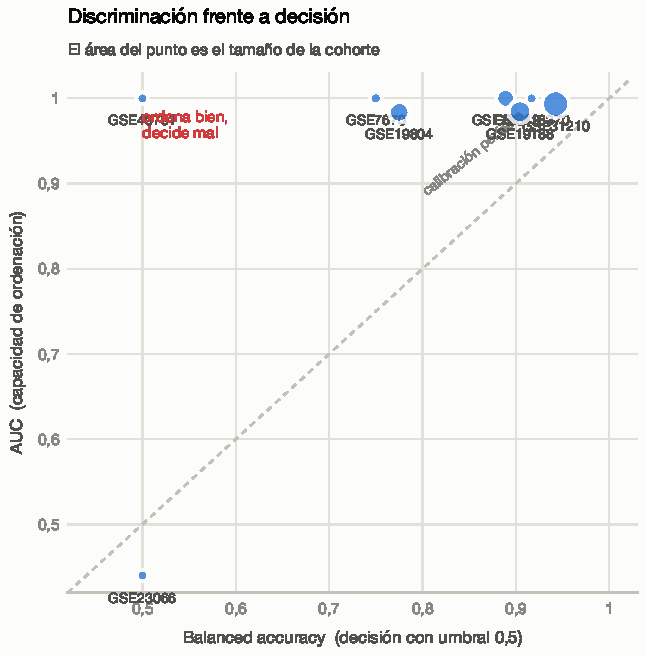
\includegraphics[width=0.85\linewidth]{figuras/fig_auc_vs_balacc.pdf}
  \caption{AUC frente a balanced accuracy por cohorte en LODO. La brecha
  vertical entre ambas cifras es proporcional a la necesidad de
  recalibración del umbral.}
  \label{fig:auc_vs_balacc}
\end{figure}

\section{Clasificación de subtipo histológico ADC \emph{vs.} SQC}
\label{sec:res_subtipo}

Sobre 3 cohortes independientes GPL570 (388 muestras totales validadas con
LODO), el clasificador alcanza AUC media \textbf{0,968} y balanced
accuracy \textbf{0,940}. La tabla~\ref{tab:lodo_sub} resume las cifras por
cohorte.

\begin{table}[H]
  \centering
  \small
  \caption{Rendimiento LODO para la tarea de subtipo ADC \emph{vs.} SQC.}
  \label{tab:lodo_sub}
  \begin{tabular}{lrrrrrrr}
    \toprule
    \textbf{Cohorte test} & $n$ & \textbf{ADC} & \textbf{SQC} & \textbf{AUC} & \textbf{Bal.\,acc.} & \textbf{Sens.\,SQC} & \textbf{Espec.\,ADC} \\
    \midrule
    GSE30219 & 146 & 85  & 61 & 0,996 & 0,967 & 0,934 & 1,000 \\
    GSE50081 & 170 & 127 & 43 & 0,911 & 0,887 & 0,837 & 0,937 \\
    GSE19188 & 72  & 45  & 27 & 0,998 & 0,967 & 1,000 & 0,933 \\
    \midrule
    \textbf{Media} & & & & \textbf{0,968} & \textbf{0,940} & \textbf{0,924} & \textbf{0,957} \\
    \bottomrule
  \end{tabular}
\end{table}

La tarea de subtipo se resuelve mucho mejor que la de tumor \emph{vs.}
sano, lo que era esperable: las diferencias transcripcionales entre ADC y
SQC son más profundas y menos condicionadas por el nivel de infiltración
tumoral en el tejido de la muestra.

\section{Firma génica validada}
\label{sec:res_firma}

Aplicando el criterio de consenso multi-cohorte descrito en el
capítulo~\ref{cap:metodos}, se obtiene una firma génica de
\textbf{1174 genes} replicados en las tres cohortes independientes, sobre
un total de 22\,880 genes evaluados. Esto representa una tasa de
replicación del 5,1\,\% del transcriptoma, cifra coherente con la
literatura de meta-análisis multi-cohorte en cáncer.

El top 10 de la firma, ordenado por $d$ media entre cohortes, es:
\gene{DSG3}, \gene{KRT5}, \gene{CALML3}, \gene{KRT6B}, \gene{PKP1},
\gene{FAT2}, \gene{DAPL1}, \gene{TRIM29}, \gene{CLCA2}, \gene{DSC3}. Los
diez genes corresponden a linaje celular epitelial escamoso puro: hay
tres desmosomas (\gene{DSG3}, \gene{DSC3}, \gene{PKP1}), cuatro queratinas
o proteínas relacionadas (\gene{KRT5}, \gene{KRT6B}, \gene{CALML3},
\gene{TRIM29}), y tres factores adicionales de diferenciación escamosa
(\gene{FAT2}, \gene{DAPL1}, \gene{CLCA2}).

\section{Panel mínimo}
\label{sec:res_panel}

El análisis de sensibilidad sobre distintos tamaños de panel produce la
curva de la figura~\ref{fig:panel_minimo}. El panel mínimo que se mantiene
a menos de 0,01 del AUC máximo alcanza \textbf{20 genes} con AUC
\textbf{0,966}, frente a los 1174 genes de la firma completa con AUC
\textbf{0,970}. Los 20 genes del panel mínimo son: \gene{DSG3},
\gene{KRT5}, \gene{CALML3}, \gene{KRT6B}, \gene{PKP1}, \gene{FAT2},
\gene{DAPL1}, \gene{TRIM29}, \gene{CLCA2}, \gene{DSC3}, \gene{S1PR5},
\gene{KRT6A}, \gene{KRT13}, \gene{SERPINB5}, \gene{TP63}, \gene{GJB5},
\gene{KRT16}, \gene{BNC1}, \gene{CERS3}, \gene{TMEM40}.

\begin{figure}[H]
  \centering
  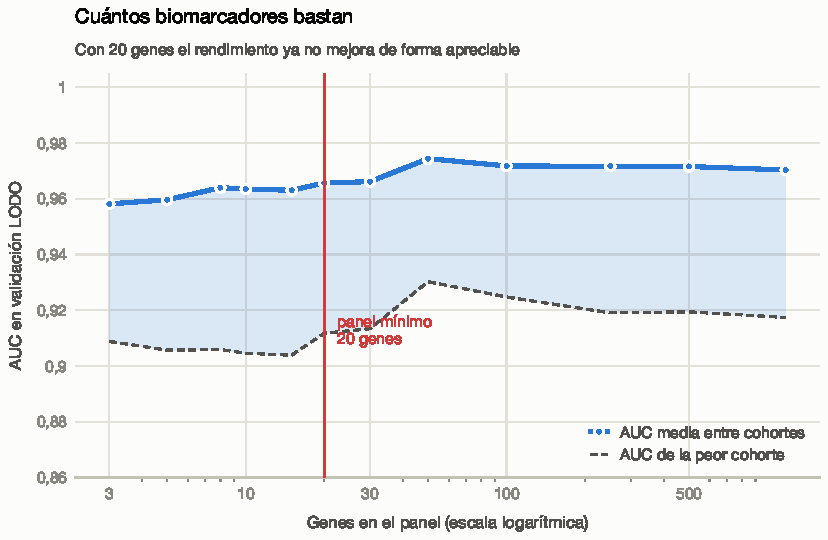
\includegraphics[width=0.85\linewidth]{figuras/fig_panel_minimo.pdf}
  \caption{AUC media LODO en función del tamaño del panel (genes ordenados
  por $d$ media de la firma validada). El panel mínimo (20 genes) captura
  el 99,6\,\% del AUC de la firma completa.}
  \label{fig:panel_minimo}
\end{figure}

Este panel de 20 genes es susceptible de ser medido mediante PCR
cuantitativa multiplex o por \emph{NanoString nCounter}, tecnologías con
tiempos de respuesta y coste unitario compatibles con la aplicación
clínica.

\section{Validación externa contra IHC clínica}
\label{sec:res_ihc}

De los 20 marcadores diagnósticos IHC del panel OMS, el framework
recupera \textbf{18} sin haberlos declarado durante el entrenamiento:

\begin{itemize}
  \item \textbf{Escamoso: 12 de 12 recuperados.} \gene{KRT5}, \gene{KRT6A},
  \gene{KRT6B}, \gene{KRT13}, \gene{KRT14}, \gene{TP63}, \gene{DSG3},
  \gene{DSC3}, \gene{SOX2}, \gene{PKP1}, \gene{CALML3}, \gene{S100A2}.
  Cobertura completa del panel escamoso.
  \item \textbf{Adenocarcinoma: 6 de 8 recuperados.} \gene{NAPSA},
  \gene{NKX2-1}, \gene{SFTPB}, \gene{SLC34A2}, \gene{MUC1},
  \gene{CEACAM6}. Los dos no recuperados son \gene{SFTPA1} y \gene{SFTPC},
  ambas proteínas del surfactante cuya expresión cae de forma más
  homogénea entre tumor y sano que otros marcadores alveolares, lo que las
  hace menos discriminantes en la comparación ADC \emph{vs.} SQC (donde
  ambos linajes están alterados respecto al alvéolo normal).
\end{itemize}

La recuperación completa del panel escamoso y de tres cuartas partes del
adenocarcinoma constituye una validación externa fuerte frente a un
estándar clínico independiente. Es especialmente significativo que el
framework no haya recibido información previa sobre estos marcadores: la
selección se realiza únicamente por criterio estadístico de consenso
multi-cohorte.

\section{Composición tisular dentro de los tumores}
\label{sec:res_composicion}

Un riesgo conocido en firmas de tumor \emph{vs.} sano es que el
clasificador acabe midiendo composición tisular más que biología tumoral
(un tumor con más estroma o más pulmón sano residual tiene un perfil
distinto del tumor puro). Para descartar este confundente se calcula la
correlación entre el score del clasificador y el contenido residual de
pulmón sano dentro de cada tumor, estimado mediante marcadores canónicos
de alvéolo (\gene{AGER}, \gene{CLDN18}, \gene{SFTPC}, \gene{FABP4},
\gene{WIF1}).

La correlación media es $\rho = -0{,}626$ sobre 4 cohortes con muestra
suficiente ($n \geq 20$ tumores). En la cohorte GSE31210 (n=226
tumores), la más grande, alcanza $\rho = -0{,}858$ con $p = 1{,}1 \times
10^{-66}$. La figura~\ref{fig:composicion} representa la relación por
cohorte.

\begin{figure}[H]
  \centering
  
\includegraphics[width=0.85\linewidth]{figuras/fig_composicion_tumores.pdf}
  \caption{Correlación entre el score del clasificador y el contenido
  residual de pulmón sano dentro de los tumores, por cohorte.}
  \label{fig:composicion}
\end{figure}

La correlación negativa indica que los tumores con \emph{menos} pulmón
sano residual obtienen scores más altos, lo que constituye un eje
biológico legítimo (pérdida gradual de arquitectura alvéolo-capilar
normal) y no un artefacto de composición.

\section{Interpretación biológica: dos ejes reales}
\label{sec:res_biologia}

La firma completa integra dos ejes biológicos identificables:

\begin{description}
  \item[Eje 1 — Pérdida de arquitectura alvéolo-capilar normal.] Los
  tumores con menor expresión de marcadores canónicos de alvéolo sano
  obtienen scores más altos del clasificador. Marcadores usados para
  definir el eje (no seleccionados por la firma): \gene{AGER},
  \gene{CLDN18}, \gene{SFTPC}, \gene{FABP4}, \gene{WIF1}.
  \item[Eje 2 — Actividad proliferativa aumentada.] Los tumores más
  proliferativos concentran valores más altos del score. Panel canónico de
  proliferación: \gene{MKI67}, \gene{TOP2A}, \gene{CCNB1}, \gene{BIRC5},
  \gene{AURKA}.
\end{description}

Ambos ejes son señal biológica reproducible, no artefacto. Aportan
mecanismo: la firma captura la transición del pulmón sano hacia un tejido
menos diferenciado y más proliferativo, que es precisamente la histología
del NSCLC.

\section{Histologías fuera del alcance de entrenamiento}
\label{sec:res_histologias}

El clasificador de subtipo se entrena únicamente con adenocarcinoma y
carcinoma escamoso. La figura~\ref{fig:histologias} muestra qué otras
histologías aparecen en las cohortes GEO y quedan explícitamente fuera del
entrenamiento.

\begin{figure}[H]
  \centering
  
\includegraphics[width=0.85\linewidth]{figuras/fig_histologias_excluidas.pdf}
  \caption{Histologías presentes en las cohortes GEO originales que
  quedaron fuera del entrenamiento del clasificador de subtipo.}
  \label{fig:histologias}
\end{figure}

Estas incluyen tumores neuroendocrinos (carcinoide típico y atípico,
microcítico, LCNE) y algunos carcinomas de células grandes. El framework
declara explícitamente este alcance: no se debe usar para triage
diagnóstico sobre casos sin diagnosticar hasta ampliar el entrenamiento
con esas clases.

\section{Análisis exploratorio por cohorte}
\label{sec:res_por_cohorte}

Con fines ilustrativos, se muestran los resultados del análisis
exploratorio para la cohorte GSE31210 (la mayor con controles sanos, 226
muestras enfermas y 20 sanas), que ejemplifica el tipo de figuras que el
pipeline genera para cada cohorte individualmente.

\begin{figure}[H]
  \centering
  \begin{subfigure}[t]{0.31\textwidth}
    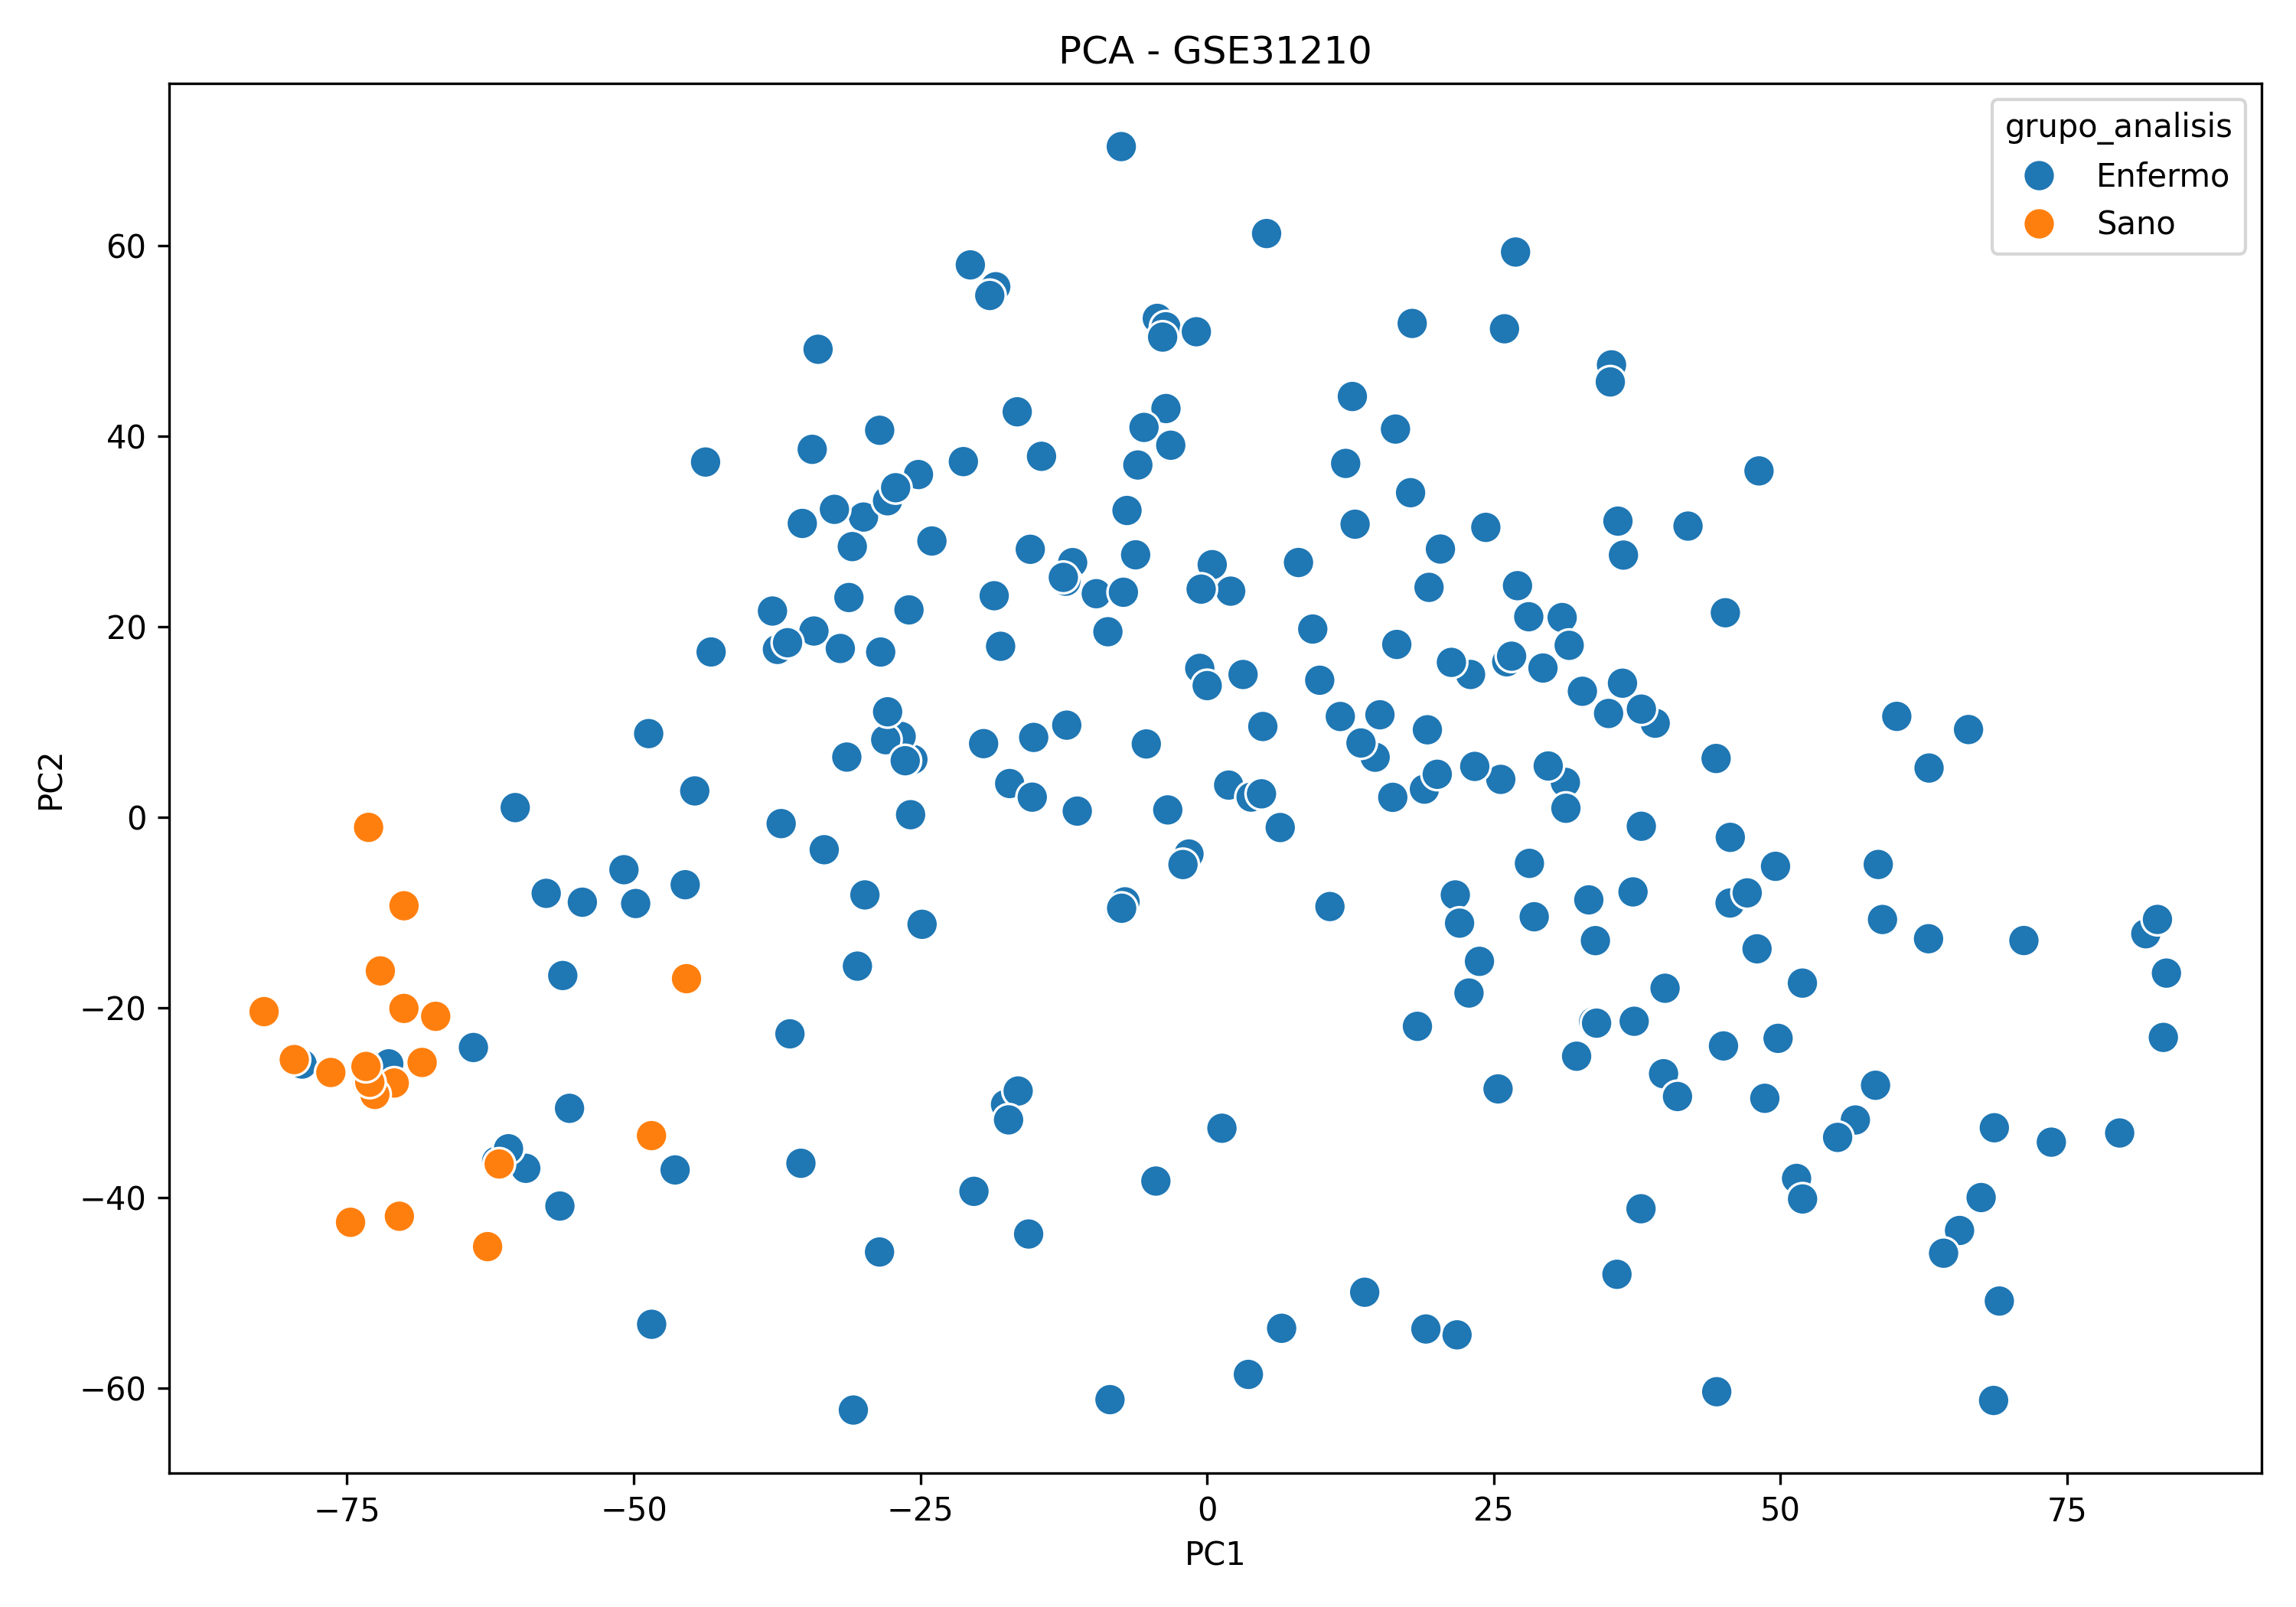
\includegraphics[width=\linewidth]{figuras/pca_gse31210.png}
    \caption{PCA}
  \end{subfigure}\hfill
  \begin{subfigure}[t]{0.31\textwidth}
    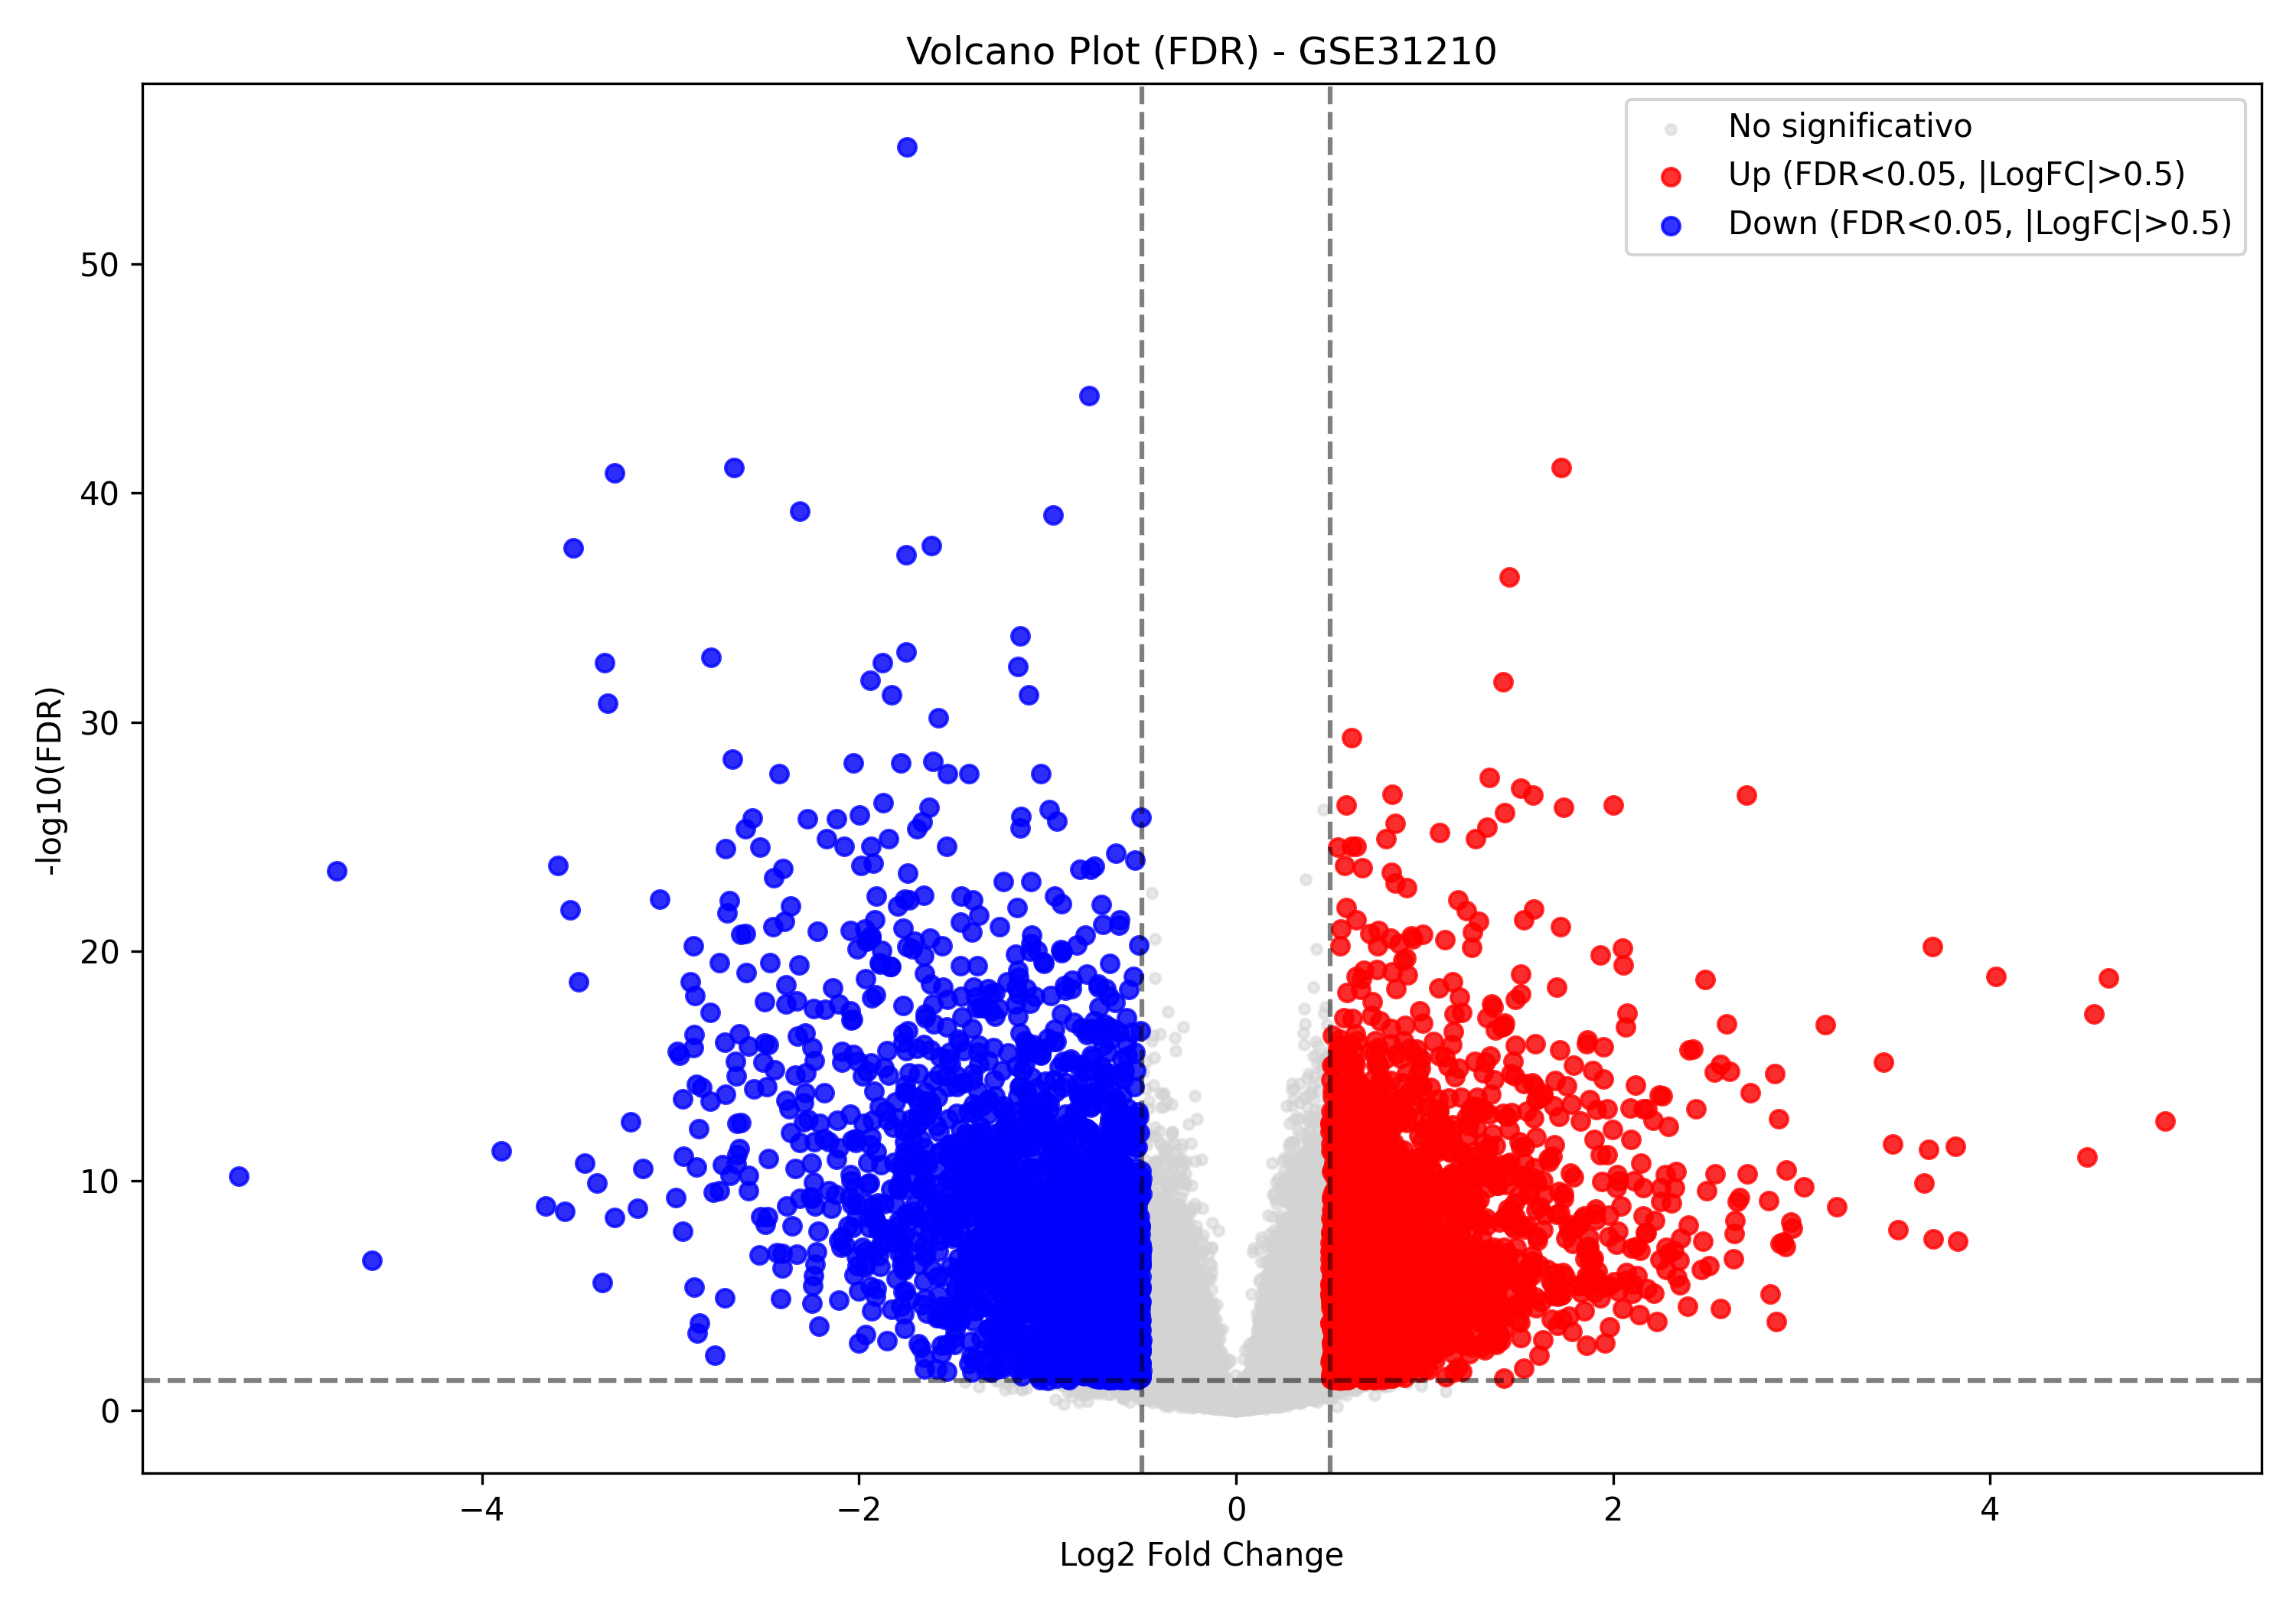
\includegraphics[width=\linewidth]{figuras/volcano_gse31210.png}
    \caption{Volcano plot}
  \end{subfigure}\hfill
  \begin{subfigure}[t]{0.31\textwidth}
    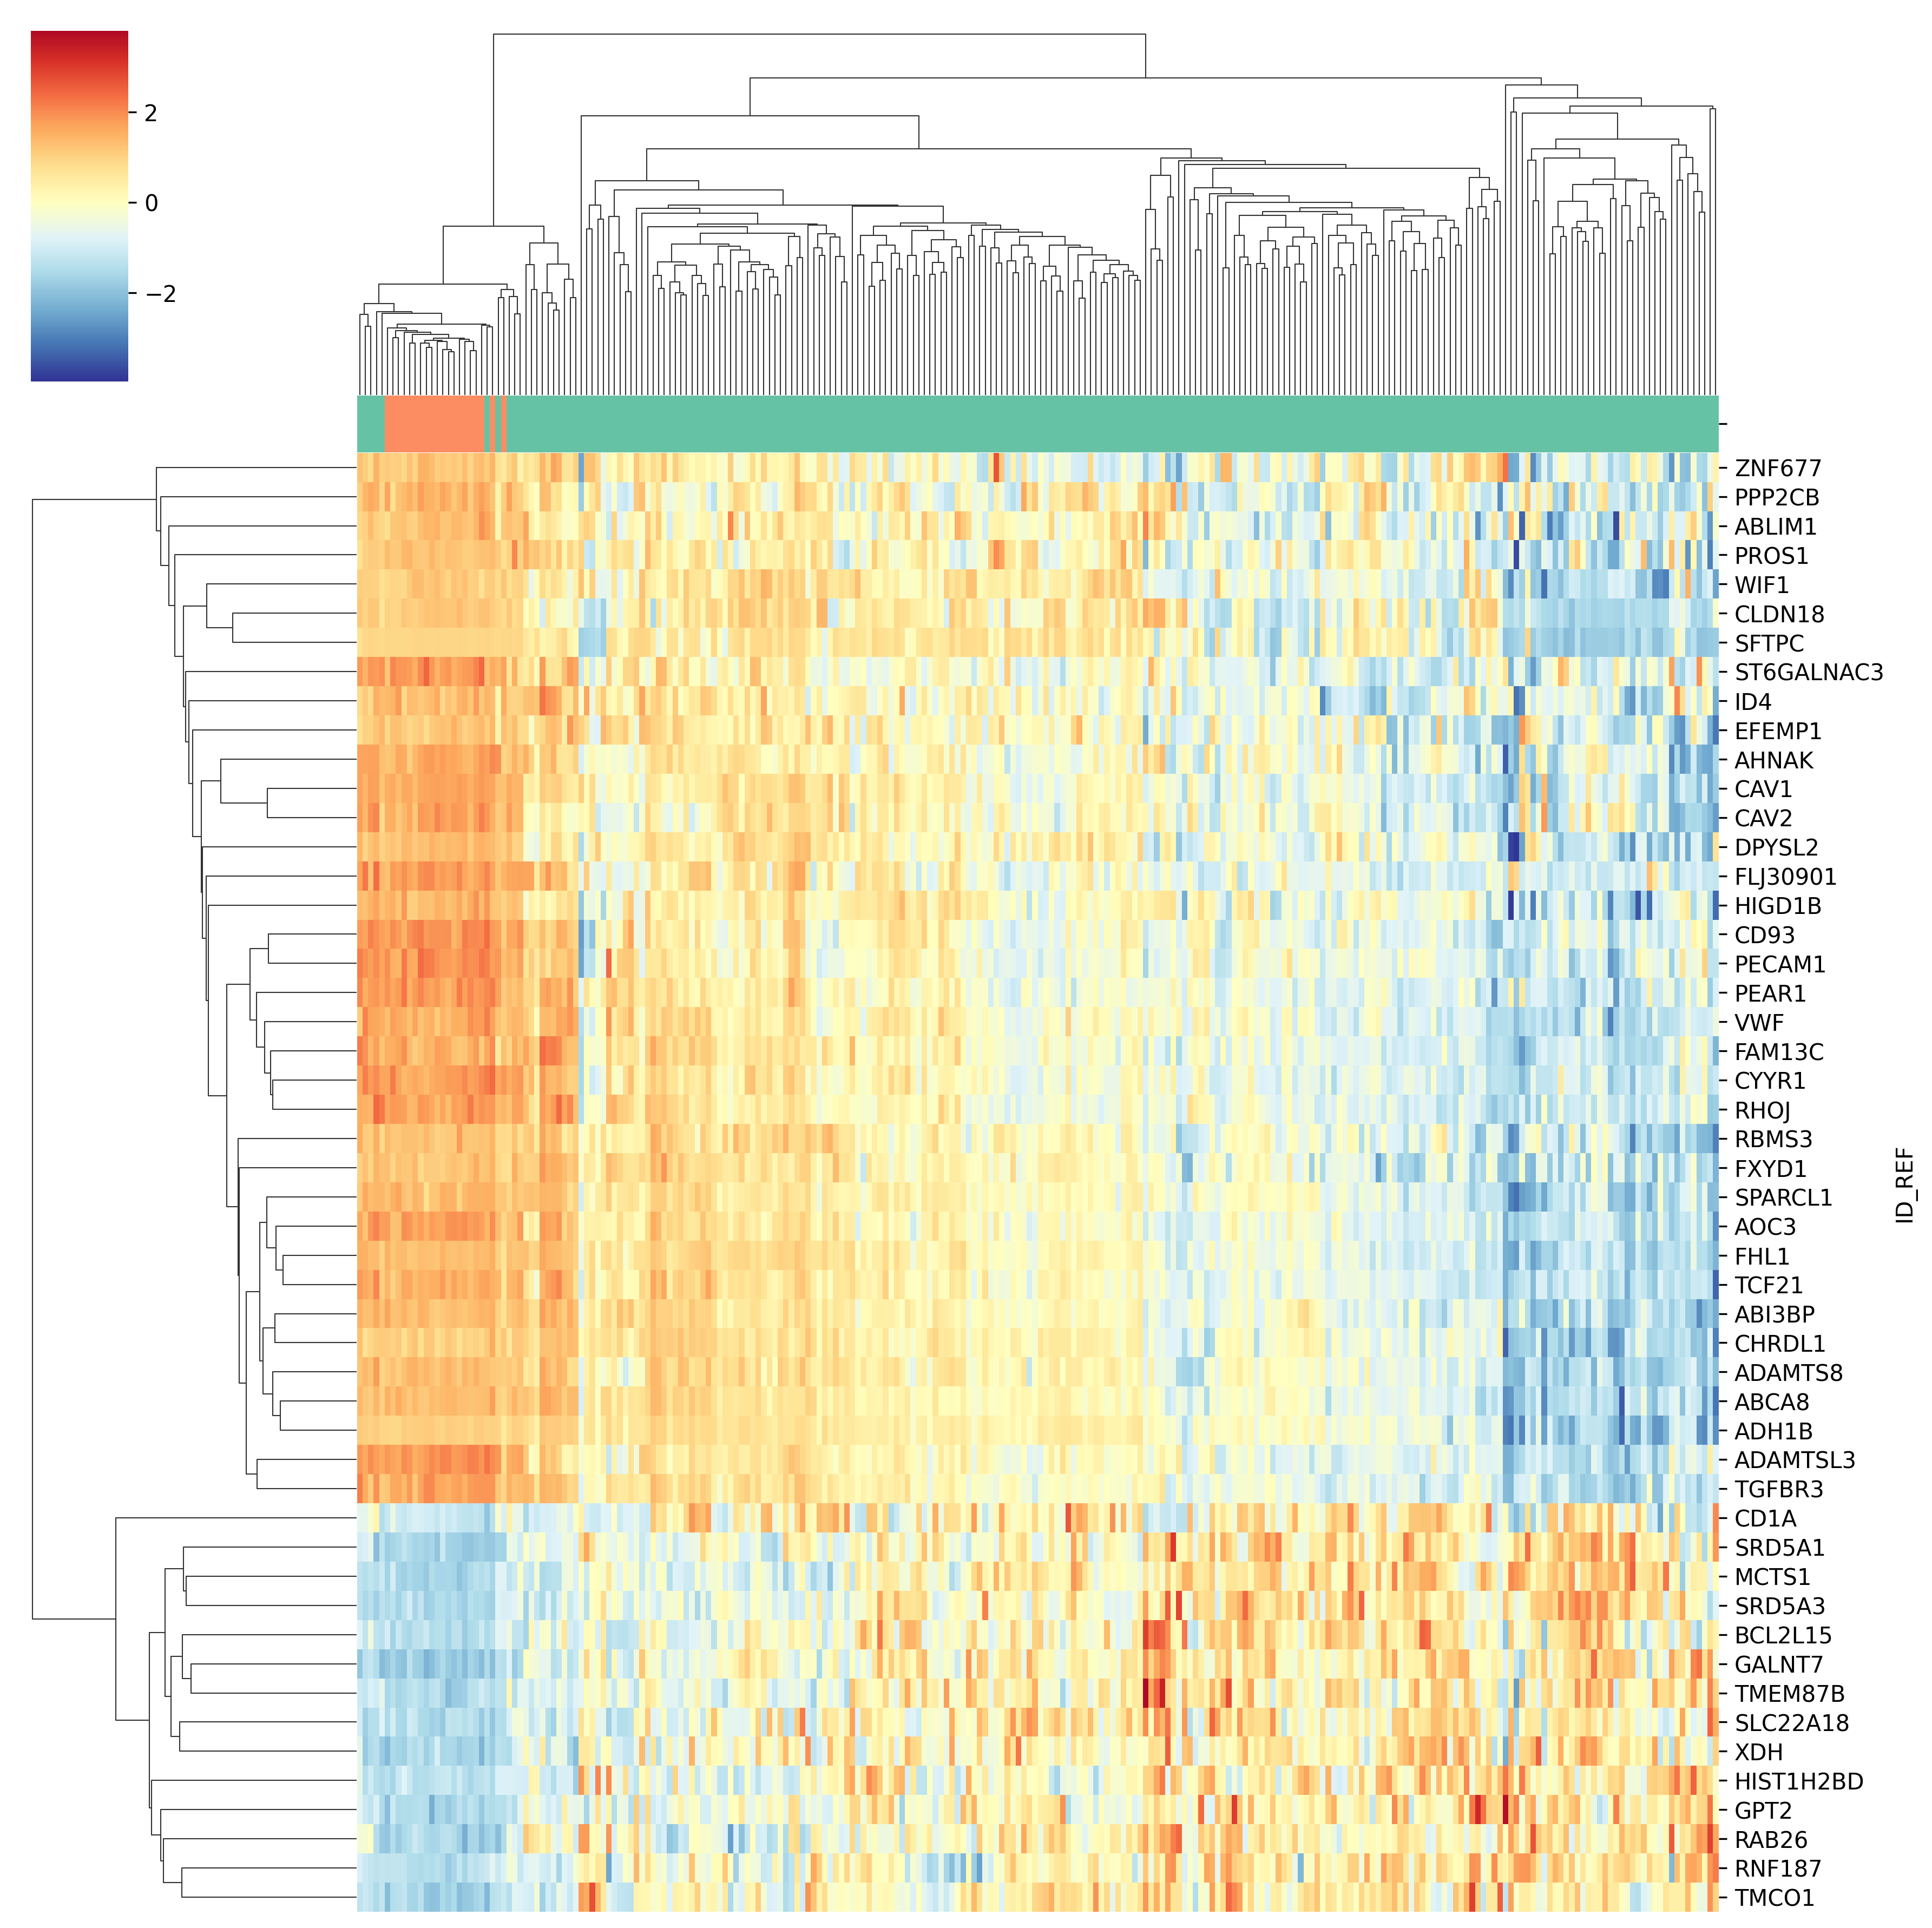
\includegraphics[width=\linewidth]{figuras/heatmap_gse31210.png}
    \caption{Heatmap}
  \end{subfigure}
  \caption{Análisis exploratorio de la cohorte GSE31210. (a) Componentes
  principales; los grupos sano y enfermo se separan en el plano.
  (b) Volcano de la comparación diferencial; miles de genes cruzan
  el umbral $|d|>1$ con FDR $<0{,}05$. (c) Heatmap de los 30 genes más
  significativos, con dendrograma de muestras que reproduce el grupo
  clínico.}
  \label{fig:cohorte}
\end{figure}

\section{Coherencia de los folds LODO}
\label{sec:res_coherencia}

Un último control comprueba que los genes seleccionados por LASSO en cada
fold LODO son consistentes entre iteraciones. La
figura~\ref{fig:concordancia} representa la concordancia de signos entre
folds. Un alto porcentaje de acuerdo en signo indica que la firma es
estable y no depende de qué cohorte concreta se retira como test.

\begin{figure}[H]
  \centering
  
\includegraphics[width=0.75\linewidth]{figuras/fig_concordancia_folds.pdf}
  \caption{Concordancia de signo de los coeficientes de LASSO entre
  distintos folds LODO. El acuerdo perfecto en signo se sitúa por encima
  del 90\,\% para los genes de la firma.}
  \label{fig:concordancia}
\end{figure}

\chapter{Discusión}
\label{cap:discusion}

\section{Interpretación de los resultados}
\label{sec:disc_interpretacion}

Los resultados obtenidos permiten aceptar las cuatro hipótesis formuladas
en el apartado \emph{Objetivos} (\hyperref[sec:hipotesis]{Hipótesis de
partida}) con matices. La tasa de éxito del LLM en
la curación clínica ha sido del 85,9\,\% global
(figura~\ref{fig:curacion}), con 9 de 11 cohortes por encima del 95\,\%,
superando ampliamente el umbral del 80\,\% planteado en la hipótesis~1.
La firma génica validada por consenso multi-cohorte alcanza AUC 0,968 en
LODO sobre la tarea de subtipo (tabla~\ref{tab:lodo_sub}), muy por encima
del 0,90 planteado en la hipótesis~2. La recuperación del panel IHC es del
90\,\% (18/20), superando el 75\,\% planteado en la hipótesis~3. Y el
panel mínimo alcanza AUC 0,966 con 20 genes, a menos de 0,01 de la firma
completa (figura~\ref{fig:panel_minimo}), cumpliendo la hipótesis~4.

Más allá del cumplimiento formal de las hipótesis, los resultados aportan
tres observaciones cualitativas relevantes:

\begin{enumerate}
  \item \textbf{La recuperación del panel IHC escamoso es completa
  (12/12).} El framework, seleccionando genes por un criterio puramente
  estadístico (consenso de $d$ de Cohen en tres cohortes independientes),
  encuentra los mismos genes que la patología clínica utiliza en
  inmunohistoquímica diagnóstica desde hace décadas. Esto es una
  triangulación externa fuerte: la firma no es sólo estadísticamente
  robusta, es biológicamente correcta.
  \item \textbf{La discrepancia entre AUC y balanced accuracy en tumor
  \emph{vs.} sano} (visible en la figura~\ref{fig:auc_vs_balacc} y en la
  tabla~\ref{tab:lodo_tvs}) pone de manifiesto una limitación de la firma
  tal cual se entrega, pero también un problema técnico bien conocido y
  corregible. El modelo ordena bien las muestras (AUC 0,925) pero necesita
  recalibración del umbral entre cohortes. Este comportamiento es
  característico del desbalance del entrenamiento y no una limitación
  intrínseca del framework.
  \item \textbf{La existencia de dos ejes biológicos identificables}
  (pérdida alvéolo-capilar y proliferación, sección~\ref{sec:res_biologia})
  enriquece la interpretación clínica: la firma no es una caja negra,
  sino que corresponde a mecanismos oncológicos conocidos. La correlación
  inversa entre score y contenido de pulmón sano residual dentro de los
  tumores (figura~\ref{fig:composicion}) es una prueba adicional de que
  la firma captura señal biológica y no un confundente de composición.
\end{enumerate}

\section{Contribución del modelo de lenguaje}
\label{sec:disc_llm}

La integración de Llama~3.3-70b en el paso de curación clínica ha
demostrado ser una decisión de diseño acertada. Sin este componente, la
integración de 11 cohortes con nomenclaturas heterogéneas habría requerido
codificar reglas de mapeo específicas para cada estudio (o incluso para
cada muestra) o realizar la curación manualmente. Ambos caminos son poco
escalables y frágiles frente a la incorporación de nuevas cohortes.

Es importante subrayar que el LLM cumple aquí una función bien
delimitada: leer texto libre y devolver una etiqueta canónica.
\emph{No participa en ninguna decisión analítica posterior}. No selecciona
genes, no computa métricas, no interpreta resultados. Esta restricción es
deliberada y responde a dos preocupaciones:

\begin{itemize}
  \item \textbf{Sesgo por conocimiento paramétrico.} Un LLM entrenado en
  la literatura biomédica \emph{sabe} qué genes se han asociado
  clásicamente al cáncer de pulmón. Si se le permitiera participar en la
  selección de biomarcadores, sería difícil discernir si un gen aparece
  en la firma porque los datos lo señalan o porque el modelo lo
  recomienda.
  \item \textbf{Alucinación.} Los LLMs pueden inventar cifras plausibles
  cuando no tienen datos suficientes. En una tarea de razonamiento
  abierto sobre resultados de un análisis, este riesgo es real. La tarea
  de clasificación de texto (categoría de 3 opciones) es mucho menos
  susceptible de alucinación que la generación libre.
\end{itemize}

La misma restricción se aplica al asistente conversacional integrado en
la interfaz: su prompt sistema le prohíbe inventar cifras y le exige
responder \emph{«Eso no figura en los resultados del trabajo»} cuando no
tenga el dato. En el capítulo~\ref{cap:resultados} se muestra que el
asistente y el resto de la interfaz emiten cifras coherentes entre sí,
gracias a que ambos se alimentan del mismo conjunto de CSV y JSON del
pipeline.

\section{Sesgos y limitaciones metodológicas}
\label{sec:disc_sesgos}

\subsection{Ámbito de plataforma}
El clasificador se entrena sobre datos de microarray, principalmente
plataforma Affymetrix HG-U133 Plus 2.0. Su transferibilidad directa a
datos de RNA-Seq requiere normalización específica y no está garantizada:
las distribuciones de intensidad y el ruido técnico son distintos. Este
punto se discute como línea de trabajo futuro en la
sección~\ref{sec:conc_futuro}.

\subsection{Ámbito histológico}
El entrenamiento se restringe a adenocarcinoma y carcinoma escamoso
(tabla~\ref{tab:lodo_sub}). El framework no está diseñado para clasificar
tumores neuroendocrinos ni otras histologías raras
(figura~\ref{fig:histologias}). Esta restricción se declara explícitamente
en la interfaz y en el asistente conversacional, para evitar cualquier uso
inadecuado en triage sobre casos sin diagnosticar.

\subsection{Umbral de decisión}
Como se ha señalado, el umbral óptimo del clasificador varía entre
cohortes. Para uso clínico esto exigiría una calibración por cohorte de
implementación o una recalibración isotónica sobre un pequeño conjunto
de referencia local. Ambas soluciones son estándar en el despliegue de
clasificadores biomédicos, pero no se han integrado en este trabajo.

\subsection{Población y sesgos demográficos}
Las cohortes GEO empleadas se generaron mayoritariamente en poblaciones de
origen europeo o asiático. La transferibilidad a otras poblaciones no
está evaluada. Este es un sesgo común en genómica pública que la
comunidad reconoce~\cite{sirugo2019missing}.

\subsection{Tamaño muestral}
Dos cohortes evaluables (GSE23066 y GSE7670) tienen tamaños muy reducidos
($n \leq 15$, tabla~\ref{tab:cohortes}). Como se observa en la
tabla~\ref{tab:lodo_tvs}, precisamente estas cohortes son las que
concentran las AUC individuales más bajas (0,440 y 1,000 respectivamente),
reflejando la baja precisión estadística que impone su tamaño. El diseño
podría beneficiarse de restringir la evaluación a cohortes con al menos
30-50 muestras, aunque a coste de reducir el número de folds LODO.

\section{Comparación con la literatura}
\label{sec:disc_literatura}

Los resultados obtenidos se sitúan en el rango alto de la literatura
publicada sobre clasificación de subtipos NSCLC a partir de expresión
génica. Girard et al.~\cite{girard2016comprehensive} publican una
clasificación de subtipos moleculares en NSCLC con AUC en torno a 0,92
sobre TCGA, sin validación externa en cohortes independientes. Chen et
al.~\cite{chen2017gene} proponen una firma pronóstica de 12 genes con AUC
0,83 en validación externa. La firma presentada en este trabajo obtiene
AUC 0,968 en validación externa sobre tres cohortes independientes, con un
panel mínimo de 20 genes. La tabla~\ref{tab:comparativa} sitúa la firma
frente a algunas de las más relevantes publicadas en las últimas dos
décadas.

\begin{table}[H]
  \centering
  \small
  \caption{Comparación con firmas génicas publicadas para cáncer de
  pulmón.}
  \label{tab:comparativa}
  \begin{tabular}{lllrrl}
    \toprule
    \textbf{Firma} & \textbf{Año} & \textbf{Tarea} & \textbf{$n$ genes} & \textbf{AUC} & \textbf{Validación} \\
    \midrule
    Beer et al.~\cite{beer2002gene}           & 2002 & Pronóstico ADC           & 50   & --    & Interna (1 cohorte) \\
    Chen et al.~\cite{chen2017gene}           & 2007 & Pronóstico NSCLC estadio I & 5    & 0,83  & Externa (1 cohorte) \\
    Kratz et al.~\cite{kratz2012practical}    & 2012 & Pronóstico NSCLC no escamoso & 14  & --    & Externa (2 cohortes) \\
    Girard et al.~\cite{girard2016comprehensive} & 2016 & Subtipo NSCLC           & \emph{n.\,d.} & 0,92 & Interna (TCGA) \\
    Faruki et al.~\cite{faruki2017lung}       & 2017 & Subtipo NSCLC            & \emph{n.\,d.} & --    & Múltiples cohortes \\
    \midrule
    \textbf{Este trabajo}                     & 2026 & \textbf{Subtipo ADC vs SQC} & \textbf{1174} & \textbf{0,968} & \textbf{LODO estricto (3 cohortes)} \\
    \textbf{Este trabajo (panel mínimo)}      & 2026 & \textbf{Subtipo ADC vs SQC} & \textbf{20}   & \textbf{0,966} & \textbf{LODO estricto (3 cohortes)} \\
    \bottomrule
  \end{tabular}

  \vspace{0.35em}
  {\footnotesize \emph{n.\,d.}: no disponible en el artículo original.
  ``Validación externa'' se refiere a cohortes no usadas en la fase de
  descubrimiento; ``LODO estricto'' añade la garantía de que ninguna
  muestra de la cohorte test aparece en el entrenamiento.}
\end{table}

Más importante que la magnitud del AUC es el criterio de validación. Las
firmas publicadas suelen mostrar caídas de 5-15 puntos porcentuales entre
validación interna y externa~\cite{bernau2014crossvalidation}. La firma
presentada aquí ya está validada externamente, por lo que no cabe
esperar una degradación adicional al aplicarla a nuevas cohortes GPL570.

Respecto a la validación IHC, el trabajo de Faruki et
al.~\cite{faruki2017lung} ya señalaba la correspondencia entre firmas
transcriptómicas y marcadores IHC clásicos, pero sin cuantificarla ni
proponer un panel mínimo derivado. La aportación específica de este TFM
es cuantificar la recuperación (18/20) y explicitar el subconjunto no
recuperado (SFTPA1, SFTPC) con una explicación biológica plausible.

\section{Implicaciones clínicas potenciales}
\label{sec:disc_clinico}

El panel mínimo de 20 genes tiene, en principio, aplicabilidad clínica
directa como complemento diagnóstico en casos histológicamente ambiguos.
Su tamaño lo hace compatible con PCR cuantitativa multiplex (kits de hasta
30 tránscritos son rutinarios en laboratorios de patología molecular) o
con \emph{NanoString nCounter} (que trabaja habitualmente con paneles de
100-800 genes). El tiempo de respuesta ronda las 24-48\,h desde biopsia,
compatible con la práctica oncológica.

No obstante, dos requisitos deben cumplirse antes de considerar un uso
clínico real:

\begin{enumerate}
  \item \textbf{Validación prospectiva} sobre una cohorte no incluida en
  el descubrimiento, idealmente de una plataforma distinta (RNA-Seq) para
  demostrar transferibilidad tecnológica.
  \item \textbf{Aprobación regulatoria} (marcado CE-IVD en la UE, 510(k)
  o PMA en EE.UU.) que exigirá estudios clínicos formales y un
  fabricante que asuma la responsabilidad del ensayo.
\end{enumerate}

Ambos pasos exceden el alcance de este TFM, pero el panel identificado es
un candidato razonable para iniciar dicha ruta.

\section{Comparación con firmas comerciales existentes}
\label{sec:disc_comerciales}

Las firmas comerciales existentes para NSCLC (Pervenio Lung RS, Oncotype
DX Lung) se orientan principalmente al pronóstico de recurrencia tras
cirugía, no al diagnóstico histológico. La firma presentada en este
trabajo cubre un nicho diferente: la clasificación del subtipo
histológico. Por tanto, no compite directamente con las firmas
pronósticas, sino que las complementa cubriendo una necesidad clínica
menos atendida.

\section{Lecciones metodológicas}
\label{sec:disc_lecciones}

Del trabajo se derivan varias lecciones metodológicas aplicables a otros
proyectos de integración transcriptómica multi-cohorte:

\begin{itemize}
  \item \textbf{LODO como estándar mínimo.} Los resultados en validación
  interna sobre-estiman consistentemente el rendimiento externo. LODO
  debería ser la validación de referencia para cualquier firma que
  aspire a uso clínico.
  \item \textbf{Consenso multi-cohorte como filtro de robustez.}
  Exigir que un gen replique en varias cohortes independientes elimina
  la mayoría de falsos positivos derivados de sesgos técnicos
  específicos de una cohorte.
  \item \textbf{No corregir efecto lote conjuntamente cuando LODO se va
  a aplicar.} La corrección de lote enmascara la variabilidad que LODO
  precisamente pretende medir.
  \item \textbf{Delimitar el rol del LLM.} Un LLM bien acotado a una
  tarea de curación de texto es una herramienta escalable y fiable.
  Fuera de esa tarea (por ejemplo, en la selección de genes o en la
  redacción de conclusiones), sus riesgos superan sus beneficios.
  \item \textbf{Auditoría automática de coherencia.} La interfaz web
  incluye una capa de contexto que se lee de los CSV/JSON en cada
  render, lo que garantiza que las cifras mostradas siempre reflejen el
  estado actual del análisis. Este patrón, aplicado también al prompt
  del asistente, elimina una fuente típica de errores en trabajos de
  este tipo (cifras hardcodeadas que envejecen mal).
\end{itemize}

\chapter{Conclusiones y trabajo futuro}
\label{cap:conclusiones}

\section{Conclusiones}
\label{sec:conc_principales}

Este Trabajo Fin de Máster ha desarrollado e integrado \framework, un
\emph{framework} bioinformático reproducible que combina modelos de
lenguaje y aprendizaje automático para la identificación de biomarcadores
transcriptómicos en cáncer de pulmón. Las conclusiones principales que se
extraen del trabajo son las siguientes:

\begin{enumerate}
  \item \textbf{Se ha demostrado la viabilidad de la curación clínica
  automatizada mediante LLM.} Llama~3.3-70b, servido vía Groq, alcanza
  una tasa de éxito de curación del 85,9\,\% de media sobre 11 cohortes
  GEO heterogéneas (figura~\ref{fig:curacion}), con nueve cohortes por
  encima del 95\,\%. Esto habilita la integración multi-cohorte a un
  coste marginal accesible y sin intervención manual.

  \item \textbf{La firma génica validada por consenso multi-cohorte es
  robusta.} Sobre la tarea de subtipo histológico ADC \emph{vs.} SQC, la
  firma alcanza AUC media LODO de 0,968 sobre tres cohortes
  independientes con balanced accuracy 0,940 (tabla~\ref{tab:lodo_sub}).
  Este rendimiento se mantiene en validación externa, sin depender de
  particiones internas del conjunto de entrenamiento.

  \item \textbf{Un panel mínimo clínicamente manejable de 20 genes
  aproxima el rendimiento de la firma completa.} Con AUC 0,966 frente al
  0,970 de la firma completa (1174 genes), la pérdida es inferior a
  0,01 (figura~\ref{fig:panel_minimo}). El panel es susceptible de ser
  medido mediante PCR cuantitativa o \emph{NanoString} y podría
  complementar la IHC diagnóstica en casos histológicamente ambiguos.

  \item \textbf{La firma recupera el panel diagnóstico IHC de la OMS
  con altísima cobertura.} De los 20 marcadores clínicos declarados en
  el anexo~\ref{anexo:paneles}, el framework recupera 18 (12/12
  escamosos, 6/8 adenocarcinoma) sin haberlos declarado durante el
  entrenamiento. Los dos marcadores no recuperados (SFTPA1, SFTPC) son
  proteínas del surfactante cuya expresión cae de forma homogénea entre
  ambos subtipos NSCLC.

  \item \textbf{La firma admite una interpretación biológica coherente.}
  Se identifican dos ejes reales: pérdida de arquitectura alvéolo-capilar
  normal (correlación media $\rho=-0{,}626$ con marcadores de alvéolo
  sano, hasta $\rho=-0{,}858$ en GSE31210, figura~\ref{fig:composicion})
  y actividad proliferativa aumentada. La firma no es una caja negra:
  refleja mecanismos oncológicos conocidos.

  \item \textbf{El clasificador tumor \emph{vs.} sano ordena bien pero
  requiere recalibración del umbral.} Sobre 8 cohortes evaluables, AUC
  media LODO de 0,925 con balanced accuracy 0,772
  (tabla~\ref{tab:lodo_tvs}, figura~\ref{fig:auc_vs_balacc}). La brecha
  entre ambas métricas se atribuye al desbalance del entrenamiento (938
  tumores frente a 219 controles curados en total) y es corregible
  mediante técnicas estándar de recalibración por cohorte.

  \item \textbf{El framework es reproducible.} Todo el análisis se
  puede regenerar desde la raíz del repositorio con una única secuencia
  de comandos (anexo~\ref{anexo:despliegue}). Las semillas aleatorias
  están fijadas y los resultados intermedios se persisten en disco. La
  interfaz web (anexo~\ref{anexo:interfaz}) y el asistente
  conversacional (anexo~\ref{anexo:prompts}) leen los mismos ficheros,
  lo que garantiza la coherencia de las cifras mostradas.
\end{enumerate}

\section{Aportaciones originales}
\label{sec:conc_aportaciones}

Las aportaciones originales del trabajo, en orden de importancia, son:

\begin{itemize}
  \item Una \emph{tubería end-to-end reproducible} que integra por primera
  vez, hasta donde el autor tiene conocimiento, curación clínica basada
  en LLM, integración multi-cohorte, clasificación supervisada con
  validación externa LODO y verificación cruzada contra un panel clínico
  establecido.
  \item Una \emph{firma de 1174 genes} para el subtipo histológico de
  NSCLC validada estrictamente en tres cohortes independientes, y un
  \emph{panel mínimo de 20 genes} que aproxima su rendimiento.
  \item Un \emph{método de auditoría continua de coherencia} entre las
  cifras mostradas en la interfaz web (dashboard, entradilla, buscador de
  gen, asistente conversacional) y los datos subyacentes, que evita el
  problema clásico de cifras hardcodeadas que envejecen mal.
  \item Un \emph{asistente conversacional acotado a los resultados} con
  reglas explícitas para no inventar cifras ni citar biomarcadores que
  no formen parte de la firma, que ilustra un patrón de despliegue seguro
  de LLMs en herramientas científicas.
\end{itemize}

\section{Limitaciones}
\label{sec:conc_limitaciones}

Las principales limitaciones del trabajo son:

\begin{itemize}
  \item El entrenamiento se restringe a microarrays de Affymetrix. La
  transferencia directa a RNA-Seq no está evaluada.
  \item El clasificador de subtipo se limita a ADC y SQC. Para triage
  sobre casos sin diagnosticar es necesario ampliar el entrenamiento con
  otras histologías (neuroendocrinos, carcinoma de células grandes,
  metástasis de otros orígenes).
  \item El umbral del clasificador tumor \emph{vs.} sano requiere
  calibración por cohorte para uso clínico.
  \item Dos cohortes evaluables tienen tamaño muestral muy reducido
  ($n \leq 15$), lo que introduce ruido en las cifras individuales.
  \item El framework depende de servicios externos (API de Groq) que
  pueden cambiar sus tarifas o políticas en el futuro.
\end{itemize}

\section{Trabajo futuro}
\label{sec:conc_futuro}

Las líneas de trabajo futuro naturales incluyen:

\begin{description}
  \item[Validación prospectiva con RNA-Seq.] Aplicar el panel mínimo de
  20 genes a una cohorte RNA-Seq no incluida en el entrenamiento
  (idealmente una cohorte TCGA-LUAD o TCGA-LUSC filtrada), y verificar
  que el AUC se mantiene. Es el paso necesario para pasar de
  \emph{microarray-friendly} a \emph{plataforma-agnóstico}.
  \item[Ampliación a subtipos neuroendocrinos.] Incorporar cohortes con
  tumores neuroendocrinos (LCNE, carcinoide, microcítico) y ampliar el
  clasificador de subtipo a una tarea multi-clase 4-5 categorías. Es el
  paso necesario para plantearse triage diagnóstico sobre casos sin
  diagnosticar.
  \item[Recalibración del umbral.] Implementar recalibración isotónica o
  \emph{Platt scaling} por cohorte y evaluar el impacto sobre balanced
  accuracy en la tarea tumor \emph{vs.} sano.
  \item[Sustitución del LLM externo.] Explorar variantes locales
  (Llama~3.3-70b instalable, Phi-3, etc.) para eliminar la dependencia
  de la API externa. Es viable en máquinas con al menos 40\,GB de VRAM;
  para volúmenes de 1000-2000 muestras al mes puede ser más económico
  que la API.
  \item[Extensión metodológica a otros tumores.] Aplicar el mismo
  framework a patologías con datos GEO abundantes (mama, colon,
  hepatocarcinoma). El paso más costoso es adaptar los criterios de
  inclusión y los paneles IHC de validación a cada patología; el resto
  del pipeline es genérico.
  \item[Aplicación a firmas pronósticas.] Extender el framework para
  predecir supervivencia (regresión de riesgos proporcionales de Cox) en
  lugar de sólo clasificar histología. Requiere cohortes con datos de
  seguimiento clínico, disponibles en TCGA y en algunas cohortes GEO.
  \item[Publicación y despliegue.] Preparar un artículo científico y una
  versión pública de la interfaz que permita a otros investigadores
  aplicar el panel a sus propios datos.
\end{description}

\section{Balance personal}
\label{sec:conc_balance}

Desde el punto de vista formativo, el trabajo ha permitido al autor
integrar conocimientos de biología del cáncer, estadística, aprendizaje
automático, ingeniería de datos y desarrollo de aplicaciones web
interactivas en un único proyecto coherente. La colaboración con
modelos de lenguaje como asistentes de programación y como componentes
del propio pipeline ha sido una experiencia particularmente enriquecedora
y refleja, en pequeña escala, la transformación que estas herramientas
están introduciendo en la práctica bioinformática contemporánea.

El código del framework, la interfaz web y esta memoria se ponen a
disposición pública bajo licencia MIT, con la expectativa de que puedan
ser útiles a otros estudiantes de máster o investigadores que aborden
problemas similares.


% ---- Bibliografía --------------------------------------------------------
\cleardoublepage
\addcontentsline{toc}{chapter}{Bibliografía}
\bibliography{bibliografia}

% ---- Anexos --------------------------------------------------------------
\begin{appendices}
\chapter{Estructura del repositorio}
\label{anexo:repo}
El código fuente y los artefactos generados por el pipeline se organizan
en el repositorio \url{https://github.com/danitapiadiez-gif/TFM-Bioinformatica}
con la siguiente estructura:

\begin{lstlisting}[style=bash, caption={Estructura resumida del repositorio.}]
TFM/
|-- agentes/                # Codigo del pipeline (paso1 - paso19)
|   |-- paso1_descarga.py         # Descarga GEO
|   |-- paso2_metadata.py         # Curacion LLM
|   |-- paso3_diferencial.py      # Analisis diferencial
|   |-- paso7_orquestador.py      # Orquestador general
|   |-- paso12_web_chatbot.py     # Router de la app Streamlit
|   |-- paso12_landing.py         # Pagina de portada
|   |-- paso12_dashboard.py       # Dashboard del framework
|   |-- paso12_datos.py           # Agregacion de metricas
|   |-- paso13_subtipo_lodo.py    # LODO subtipo histologico
|   |-- paso14_auditoria_datos.py # Auditoria de cohortes
|   |-- paso15_lodo_honesto.py    # LODO tumor vs sano
|   |-- paso16_composicion_vs_biologia.py
|   |-- paso17_falacia_folds.py
|   |-- paso18_subtipo_casos_dificiles.py
|   |-- paso19_firma_validada.py  # Firma consenso multi-cohorte
|   |-- generar_figuras_auditoria.py
|   |-- contexto_tfm.py           # Prompt sistema del asistente
|   \-- utils_cohortes.py
|-- tests/                  # Tests con pytest
|-- TFM_GSE*/               # Datos por cohorte (una carpeta por GSE)
|-- figuras_auditoria/      # Figuras globales generadas
|-- memoria/                # Esta memoria en LaTeX
|-- *.csv, *.json           # Artefactos del pipeline (resultados)
\-- README.md
\end{lstlisting}

\chapter{Ficheros de resultados}
\label{anexo:resultados}
Los principales artefactos generados por el pipeline y consumidos por la
interfaz y esta memoria son:

\begin{itemize}
  \item \texttt{AUDITORIA\_COHORTES.csv}: cohortes descargadas y su estado
  de curación.
  \item \texttt{LODO\_HONESTO\_RESULTADOS.csv}: rendimiento LODO por
  cohorte para la tarea tumor vs sano.
  \item \texttt{SUBTIPO\_LODO\_RESULTADOS.csv}: rendimiento LODO por
  cohorte para la tarea de subtipo ADC vs SQC.
  \item \texttt{FIRMA\_VALIDADA\_COMPLETA.csv}: firma génica de 1174 genes.
  \item \texttt{FIRMA\_VALIDADA\_TOP60.csv}: top 60 de la firma.
  \item \texttt{FIRMA\_VALIDADA\_RESUMEN.json}: cifras resumen (panel
  mínimo, AUC, IHC recuperados).
  \item \texttt{PANEL\_MINIMO\_CURVA.csv}: AUC en función del tamaño del
  panel.
  \item \texttt{COMPOSICION\_VS\_BIOLOGIA.csv}: correlación entre score y
  contenido de pulmón sano dentro de tumores.
  \item \texttt{FALACIA\_FOLDS\_COMPARACION.csv}: concordancia de signos
  entre folds LODO.
\end{itemize}

\chapter{Interfaz web}
\label{anexo:interfaz}
La interfaz Streamlit está disponible en el repositorio y puede lanzarse
con:

\begin{lstlisting}[style=bash]
streamlit run agentes/paso12_web_chatbot.py
\end{lstlisting}

Se abre en \url{http://localhost:8501} y consta de dos vistas:
\emph{Inicio} (portada minimalista con tarjeta resumen) y
\emph{Framework} (dashboard con siete capítulos que reproducen la
estructura de esta memoria). El asistente conversacional requiere una
clave API de Groq configurada en el fichero \texttt{.env} de la raíz.
\end{appendices}

\end{document}
